\documentclass[oneside]{book}
\usepackage[latin1]{inputenc}
\usepackage[reqno]{amsmath}
\usepackage{makeidx,graphicx}
\makeindex
\renewcommand{\chaptername}{Article}
\DeclareMathOperator{\Sin}{Sin}
\begin{document}
\thispagestyle{empty}
\small
\begin{verbatim}
Project Gutenberg's Vector Analysis and Quaternions, by Alexander Macfarlane

This eBook is for the use of anyone anywhere at no cost and with
almost no restrictions whatsoever.  You may copy it, give it away or
re-use it under the terms of the Project Gutenberg License included
with this eBook or online at www.gutenberg.net


Title: Vector Analysis and Quaternions

Author: Alexander Macfarlane

Release Date: October 5, 2004 [EBook #13609]

Language: English

Character set encoding: TeX

*** START OF THIS PROJECT GUTENBERG EBOOK VECTOR ANALYSIS AND QUATERNIONS ***




Produced by David Starner, Joshua Hutchinson, John Hagerson, and the 
Project Gutenberg On-line Distributed Proofreaders.





\end{verbatim}
\normalsize
\newpage

\frontmatter

\begin{center}
\noindent \Large MATHEMATICAL MONOGRAPHS.

\bigskip\footnotesize{EDITED BY} \\
\normalsize \textsc{MANSFIELD MERRIMAN and ROBERT S. WOODWARD.}

\bigskip\bigskip\huge
No. 8.

\bigskip\bigskip\huge VECTOR ANALYSIS \\
\bigskip\footnotesize \textsc{and} \\
\bigskip\huge QUATERNIONS.

\bigskip\bigskip\footnotesize \textsc{by} \\
\bigskip \large ALEXANDER MACFARLANE, \\
\footnotesize\textsc{Secretary of International Association for
Promoting the Study of Quaternions.} \\

\bigskip\bigskip\normalsize NEW YORK: \\
\medskip JOHN WILEY \& SONS. \\
\medskip \textsc{London: CHAPMAN \& HALL, Limited.} \\
\medskip 1906.
\end{center}

\bigskip\bigskip
\scriptsize \noindent \textsc{Transcriber's Notes:} \emph{This
material was originally published in a book by Merriman and Woodward
titled \emph{Higher Mathematics}. I believe that some of the page
number cross-references have been retained from that presentation of
this material.}

\emph{I did my best to recreate the index.} \normalsize

\newpage

\fbox{\parbox{11cm}{
\begin{center}
\textbf{MATHEMATICAL MONOGRAPHS.} \\
\footnotesize\textsc{edited by}\normalsize \\
\textbf{Mansfield Merriman and Robert S. Woodward.} \\
\smallskip \footnotesize \textbf{Octavo. Cloth. \$1.00 each.}

\bigskip
\textbf{No. 1. History of Modern Mathematics.} \\
By \textsc{David Eugene Smith.}

\smallskip
\textbf{No. 2. Synthetic Projective Geometry.} \\
By \textsc{George Bruce Halsted.}

\smallskip
\textbf{No. 3. Determinants.} \\
By \textsc{Laenas Gifford Weld.}

\smallskip
\textbf{No. 4. Hyperbolic Functions.} \\
By \textsc{James McMahon.}

\smallskip
\textbf{No. 5. Harmonic Functions.} \\
By \textsc{William E. Byerly.}

\smallskip
\textbf{No. 6. Grassmann's Space Analysis.} \\
By \textsc{Edward W. Hyde.}

\smallskip
\textbf{No. 7. Probability and Theory of Errors.} \\
By \textsc{Robert S. Woodward.}

\smallskip
\textbf{No. 8. Vector Analysis and Quaternions.} \\
By \textsc{Alexander Macfarlane.}

\smallskip
\textbf{No. 9. Differential Equations.} \\
By \textsc{William Woolsey Johnson.}

\smallskip
\textbf{No. 10. The Solution of Equations.} \\
By \textsc{Mansfield Merriman.}

\smallskip
\textbf{No. 11. Functions of a Complex Variable.} \\
By \textsc{Thomas S. Fiske.}

\normalsize \bigskip PUBLISHED BY \\
\smallskip \textbf{JOHN WILEY \& SONS, Inc., NEW YORK. \\
CHAPMAN \& HALL, Limited, LONDON.}
\end{center}}}

\chapter{Editors' Preface}

The volume called Higher Mathematics, the first edition of which was
published in 1896, contained eleven chapters by eleven authors, each
chapter being independent of the others, but all supposing the
reader to have at least a mathematical training equivalent to that
given in classical and engineering colleges. The publication of that
volume is now discontinued and the chapters are issued in separate
form. In these reissues it will generally be found that the
monographs are enlarged by additional articles or appendices which
either amplify the former presentation or record recent advances.
This plan of publication has been arranged in order to meet the
demand of teachers and the convenience of classes, but it is also
thought that it may prove advantageous to readers in special lines
of mathematical literature.

It is the intention of the publishers and editors to add other
monographs to the series from time to time, if the call for the same
seems to warrant it. Among the topics which are under consideration
are those of elliptic functions, the theory of numbers, the group
theory, the calculus of variations, and non-Euclidean geometry;
possibly also monographs on branches of astronomy, mechanics, and
mathematical physics may be included. It is the hope of the editors
that this form of publication may tend to promote mathematical study
and research over a wider field than that which the former volume
has occupied.

\medskip \footnotesize December, 1905. \normalsize

\chapter{Author's Preface}

Since this Introduction to Vector Analysis and Quaternions was first
published in 1896, the study of the subject has become much more
general; and whereas some reviewers then regarded the analysis as a
luxury, it is now recognized as a necessity for the exact student of
physics or engineering. In America, Professor Hathaway has published
a Primer of Quaternions (New York, 1896), and Dr. Wilson has
amplified and extended Professor Gibbs' lectures on vector analysis
into a text-book for the use of students of mathematics and physics
(New York, 1901). In Great Britain, Professor Henrici and Mr. Turner
have published a manual for students entitled Vectors and Rotors
(London, 1903); Dr. Knott has prepared a new edition of Kelland and
Tait's Introduction to Quaternions (London, 1904); and Professor
Joly has realized Hamilton's idea of a Manual of Quaternions
(London, 1905). In Germany Dr. Bucherer has published Elemente der
Vektoranalysis (Leipzig, 1903) which has now reached a second
edition.\index{Bibliography}

Also the writings of the great masters have been rendered more
accessible. A new edition of Hamilton's classic, the Elements of
Quaternions, has been prepared by Professor Joly (London, 1899,
1901); Tait's Scientific Papers have been reprinted in collected
form (Cambridge, 1898, 1900); and a complete edition of Grassmann's
mathematical and physical works has been edited by Friedrich Engel
with the assistance of several of the eminent mathematicians of
Germany (Leipzig, 1894--). In the same interval many papers,
pamphlets, and discussions have appeared. For those who desire
information on the literature of the subject a Bibliography has been
published by the Association for the promotion of the study of
Quaternions and Allied Mathematics (Dublin, 1904).

There is still much variety in the matter of notation, and the
relation of Vector Analysis to Quaternions is still the subject of
discussion (see Journal of the Deutsche Mathematiker-Vereinigung for
1904 and 1905).

\medskip \footnotesize \textsc{Chatham, Ontario, Canada,}
December, 1905. \normalsize

\tableofcontents

%%  1. INTRODUCTION
%%  2. ADDITION OF COPLANAR VECTORS
%%  3. PRODUCTS OF COPLANAR VECTORS
%%  4. COAXIAL QUATERNIONS
%%  5. ADDITION OF VECTORS IN SPACE
%%  6. PRODUCT OF TWO VECTORS
%%  7. PRODUCT OF THREE VECTORS
%%  8. COMPOSITION OF LOCATED QUANTITIES
%%  9. SPHERICAL TRIGONOMETRY
%% 10. COMPOSITION OF ROTATIONS
%% INDEX

\mainmatter

\chapter{Introduction.}

By ``Vector Analysis'' is meant a space analysis in which the vector
is the fundamental idea; by ``Quaternions'' is meant a
space-analysis in which the quaternion is the fundamental idea.%
\index{Quaternions!definion of}%
\index{Quaternions!relation to vector analysis}%
\index{Space-analysis}%
\index{Vector analysis!definition of}%
\index{Vector analysis!relation to Quaternions} They are in truth
complementary parts of one whole; and in this chapter they will be
treated as such, and developed so as to harmonize with one another
and with the Cartesian Analysis\footnote{For a discussion of the
relation of
Vector Analysis to Quaternions, see Nature, 1891--1893.}.%
\index{Cartesian analysis} The subject to be treated is the analysis
of quantities in space, whether they are vector in nature, or
quaternion in nature, or of a still different nature, or are of such
a kind that they can be adequately represented by space quantities.

Every proposition about quantities in space ought to remain true
when restricted to a plane; just as propositions about quantities in
a plane remain true when restricted to a straight line. Hence in the
following articles the ascent to the algebra of space%
\index{Algebra!of space} is made through the intermediate algebra of
the plane\index{Algebra!of the plane}. Arts.\ 2--4 treat of the more
restricted analysis, while Arts.\ 5--10 treat of the general
analysis.

This space analysis is a universal Cartesian analysis, in the same
manner as algebra is a universal arithmetic. By providing an
explicit notation for directed quantities, it enables their general
properties to be investigated independently of any particular system
of coordinates, whether rectangular, cylindrical, or polar. It also
has this advantage that it can express the directed quantity by a
linear function of the coordinates, instead of in a roundabout way
by means of a quadratic function.%
\index{Space-analysis!advantage over Cartesian analysis}

The different views of this extension of analysis which have been
held by independent writers are briefly indicated by the titles of
their works:\index{Bibliography}

\small\begin{itemize}
\item Argand, Essai sur une mani�re de repr�senter les
quantit�s imaginaires dans les constructions g�om�triques, 1806.

\item Warren, Treatise on the geometrical representation of the
square roots of negative quantities, 1828.

\item Moebius, Der barycentrische Calcul, 1827.

\item Bellavitis, Calcolo delle Equipollenze, 1835.

\item Grassmann, Die lineale Ausdehnungslehre, 1844.

\item De~Morgan, Trigonometry and Double Algebra, 1849.

\item O'Brien, Symbolic Forms derived from the conception of the
translation of a directed magnitude. Philosophical Transactions,
1851.

\item Hamilton, Lectures on Quaternions, 1853, and Elements of
Quaternions, 1866.

\item Tait, Elementary Treatise on Quaternions, 1867.

\item Hankel, Vorlesungen �ber die complexen Zahlen und ihre
Functionen, 1867.

\item Schlegel, System der Raumlehre, 1872.

\item Ho�el, Th�orie des quantit�s complexes, 1874.

\item Gibbs, Elements of Vector Analysis, 1881--4.

\item Peano, Calcolo geometrico, 1888.

\item Hyde, The Directional Calculus, 1890.

\item Heaviside, Vector Analysis, in ``Reprint of Electrical
Papers,'' 1885--92.

\item Macfarlane, Principles of the Algebra of Physics, 1891. Papers
on Space Analysis, 1891--3.
\end{itemize}

An excellent synopsis is given by Hagen in the second volume of his
``Synopsis der h�heren Mathematik.'' \normalsize

\chapter{Addition of Coplanar Vectors.}

By a ``vector'' is meant a quantity which has magnitude and
direction.\index{Vector!definition of} It is graphically represented
by a line whose length represents the magnitude on some convenient
scale, and whose direction coincides with or represents the
direction of the vector. Though a vector is represented by a line,
its physical dimensions may be different from that of a line.
Examples are a linear velocity which is of one dimension in length,
a directed area which is of two dimensions in length, an axis which
is of no dimensions in length.

A vector will be denoted by a capital italic letter, as
$B$,\footnote{This notation is found convenient by electrical
writers in order to harmonize with the Hospitalier system of symbols
and abbreviations.\index{Hospitalier system}} its magnitude by a
small italic letter, as $b$, and its direction by a small Greek
letter, as $\beta$.\index{Notation for vector}%
\index{Vector!dimensions of}%
\index{Vector!notation for} For example, $B = b\beta$, $R = r\rho$.
Sometimes it is necessary to introduce a dot or a mark $\angle$ to
separate the specification of the direction from the expression for
the magnitude;\footnote{The dot was used for this purpose in the
author's Note on Plane Algebra, 1883; Kennelly has since used
$\angle$ for the same purpose in his electrical
papers.\index{Kennelly's notation}}%
\index{Meaning!of dot}%
\index{Meaning!of $\angle$} but in such simple expressions as the
above, the difference is sufficiently indicated by the difference of
type. A system of three mutually rectangular axes will be indicated,
as usual, by the letters $i$, $j$, $k$.\index{Unit-vector}

The analysis of a vector here supposed is that into magnitude and
direction. According to Hamilton and Tait and other writers on
Quaternions, the vector is analyzed into tensor and unit-vector,
which means that the tensor is a mere ratio destitute of dimensions,
while the unit-vector is the physical magnitude.%
\index{Hamilton's!analysis of vector}%
\index{Tait's analysis of vector} But it will be found that the
analysis into magnitude and direction is much more in accord with
physical ideas, and explains readily many things which are difficult
to explain by the other analysis.

A vector quantity may be such that its components have a common
point of application and are applied simultaneously;%
\index{Simultaneous components}%
\index{Vector!simultaneous} or it may be such that its components
are applied in succession, each component
starting from the end of its predecessor.%
\index{Successive components}%
\index{Vector!successive} An example of the former is found in two
forces applied simultaneously at the same point, and an example of
the latter in two rectilinear displacements made in succession to
one another.

\begin{center}
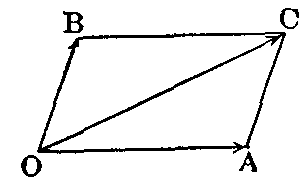
\includegraphics[width=40mm]{fig01.png}
\end{center}

\smallskip Composition of Components having a common Point of
Application.%
\index{Composition!of two simultaneous components}%
\index{Parallelogram of simultaneous components}%
\index{Simultaneous components!composition of}%
\index{Simultaneous components!parallelogram of}---Let $OA$ and $OB$
represent two vectors of the same kind simultaneously applied at the
point $O$. Draw $BC$ parallel to $OA$, and $AC$ parallel to $OB$,
and join $OC$. The diagonal $OC$ represents in magnitude and
direction and point of application the resultant of $OA$ and $OB$.
This principle was discovered with reference to force, but it
applies to any vector quantity coming under the above conditions.

Take the direction of $OA$ for the initial direction; the direction
of any other vector will be sufficiently denoted by the angle round
which the initial direction has to be turned in order to coincide
with it. Thus $OA$ may be denoted by $f_1\underline{/0}$, $OB$ by
$f_2\underline{/\theta_2}$, $OC$ by $f\underline{/\theta}$. From the
geometry of the figure it follows that
\begin{gather*}
f^2 = f_1^2 + f_2^2 + 2f_1f_2 \cos \theta_2 \\
\intertext{and}
\tan \theta =\frac{f_2\sin\theta_2}{f_1 + f_2\cos\theta_2}; \\
\intertext{hence}
OC = \sqrt{f_1^2 + f_2^2 + 2f_1f_2\cos\theta^2}
  \underline{\left/\tan^{-1}
    \frac{f_2\sin \theta_2}{f_1 + f_2\cos\theta^2}\right.}.
\end{gather*}

\smallskip Example.---Let the forces applied at a point be
$2\underline{/0^{\circ}}$ and $3\underline{/60^{\circ}}$. Then the
resultant is $\sqrt{4 + 9 + 12 \times \frac{1}{2}}\,
\underline{\left/\tan^{-1}\frac{3\sqrt{3}}{7}\right.} =
4.36\underline{/36^{\circ}\,30'}$.

\smallskip If the first component is given as
$f_1\underline{/\theta_1}$, then we have the more symmetrical
formula
\begin{equation*}
OC = \sqrt{f_1^2 + f_2^2 + 2f_1f_2\cos(\theta_2 - \theta_1)}\,
     \underline{\left/\tan^{-1} \frac{f_1\sin\theta_1 +
       f_2\sin\theta_2}{f_1\cos\theta_1 + f_2\cos\theta_2}\right.}.
\end{equation*}

When the components are equal, the direction of the resultant
bisects the angle formed by the vectors; and the magnitude of the
resultant is twice the projection of either component on the
bisecting line. The above formula reduces to
\begin{equation*}
OC = 2f_1\cos\frac{\theta_2}{2}
  \underline{\left/\frac{\theta_2}{2}\right.}.
\end{equation*}

\smallskip Example.---The resultant of two equal alternating
electromotive forces which differ $120^\circ$ in phase is equal in
magnitude to either and has a phase of $60^\circ$.

\begin{center}
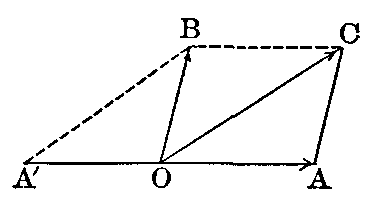
\includegraphics[width=40mm]{fig02.png}
\end{center}

\smallskip Given a vector and one component, to find the other
component.---Let $OC$ represent the resultant, and $OA$ the
component. Join $AC$ and draw $OB$ equal and parallel to $AC$. The
line $OB$ represents the component required, for it is the only line
which combined with $OA$ gives $OC$ as resultant. The line $OB$ is
identical with the diagonal of the parallelogram formed by $OC$ and
$OA$ reversed; hence the rule is, ``Reverse the direction of the
component, then compound it with the given resultant to find the
required component.'' Let $f\underline{/\theta}$ be the vector and
$f_1\underline{/0}$ one component; then the other component is
\begin{equation*}
f_2\underline{/\theta_2} = \sqrt{f^2 + f_1^2 - 2ff_1\cos\theta}
  \underline{\left/\tan^{-1}
             \frac{f\sin\theta}{-f_1 + f\cos\theta}\right.}
\end{equation*}

\begin{center}
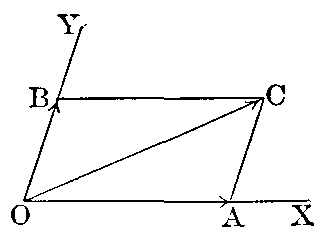
\includegraphics[width=40mm]{fig03.png}
\end{center}

\smallskip Given the resultant and the directions of the two
components, to find the magnitude of the components.%
\index{Resolution!of a vector}%
\index{Simultaneous components!resolution of}---The resultant is
represented by $OC$, and the directions by $OX$ and $OY$. From C
draw $CA$ parallel to $OY$, and $CB$ parallel to $OX$; the lines
$OA$ and $OB$ cut off represent the required components. It is
evident that $OA$ and $OB$ when compounded produce the given
resultant $OC$, and there is only one set of two components which
produces a given resultant; hence they are the only pair of
components having the given directions.

\smallskip Let $f\underline{/\theta}$ be the vector and
$\underline{/\theta_1}$ and $\underline{/\theta_2}$ the given
directions. Then
\begin{align*}
f_1 + f_2\cos(\theta_2 - \theta_1) &= f\cos(\theta - \theta_1), \\
f_1\cos(\theta_2 - \theta_1) + f_2 &= f\cos(\theta_2 - \theta),
\end{align*}
from which it follows that
\begin{equation*}
f_1 = f\frac{ \{\cos(\theta - \theta_1)
        - \cos(\theta_2 - \theta)\cos(\theta_2 - \theta_1)\} }
      {1 - \cos^2(\theta_2 - \theta_1)}.
\end{equation*}

For example, let $100\underline{/60^\circ}$,
$\underline{/30^\circ}$, and $\underline{/90^\circ}$ be given; then
\begin{equation*}
f_1 = 100 \frac{\cos 30^\circ}{1 + \cos 60^\circ} .
\end{equation*}

\begin{center}
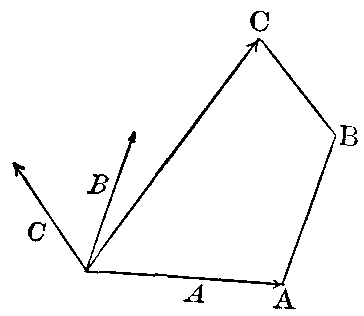
\includegraphics[width=40mm]{fig04.png}
\end{center}

\smallskip Composition of any Number of Vectors applied at a common
Point.%
\index{Composition!of any number of simultaneous components}%
\index{Polygon of simultaneous components}%
\index{Simultaneous components!polygon of}---The resultant may be
found by the following graphic construction: Take the vectors in any
order, as $A$, $B$, $C$. From the end of $A$ draw $B'$ equal and
parallel to $B$, and from the end of $B'$ draw $C'$ equal and
parallel to $C$; the vector from the beginning of $A$ to the end of
$C'$ is the resultant of the given vectors. This follows by
continued application of the parallelogram construction. The
resultant obtained is the same, whatever the order; and as the order
is arbitrary, the area enclosed has no physical meaning.

The result may be obtained analytically as follows:

Given
\begin{gather*}
f_1\underline{/\theta_1} + f_2\underline{/\theta_2} +
  f_3\underline{/\theta_3} + \cdots + f_n\underline{/\theta_n}. \\
\intertext{Now}
f_1\underline{/\theta_1} = f_1\cos\theta_1\underline{/0} +
  f_1\sin\theta_1\underline{\left/ \frac{\pi}{2}\right.}. \\
\intertext{Similarly}
f_2\underline{/\theta_2} = f_2\cos\theta_2\underline{/0}
  + f_2\sin\theta_2\underline{\left/ \frac{\pi}{2}\right.}. \\
\intertext{and}
f_n\underline{/\theta_n} = f_n\cos\theta_n\underline{/0} +
  f_n\sin\theta_n\underline{\left/ \frac{\pi}{2}\right.}. \\
\intertext{Hence}
\begin{align*}
\sum\Bigl\lbrace f\underline{/\theta} \Bigr\rbrace & =
  \Bigl\lbrace \sum f\cos\theta \Bigr\rbrace \underline{/0} +
  \Bigl\lbrace \sum f\sum\theta \Bigr\rbrace
    \underline{\left/ \frac{\pi}{2}\right.} \\
& =\sqrt{\left( \sum f\cos\theta \right)^2 +
     \left( \sum f\sin\theta \right )^2} \cdot
  \tan^{-1}\frac{\sum f\sin\theta}{\sum f\cos\theta}.
\end{align*}
\end{gather*}

In the case of a sum of simultaneous vectors applied at a common
point, the ordinary rule about the transposition of a term in an
equation holds good. For example, if $A + B + C = 0$, then $A + B =
-C$, and $A + C = -B$, and $B + C = -A$, etc. This is permissible
because there is no real order of succession among the given
components.\footnote{ This does not hold true of a sum of vectors
having a real order of succession. It is a mistake to attempt to
found space-analysis upon arbitrary formal laws; the fundamental
rules must be made to express universal properties of the thing
denoted. In this chapter no attempt is made to apply formal laws to
directed quantities. What is attempted is an analysis of these
quantities.}\index{Space-analysis!foundation of}

\begin{center}
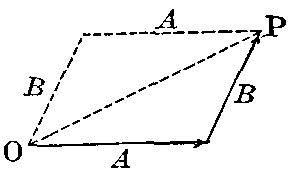
\includegraphics[width=50mm]{fig05.png} \qquad
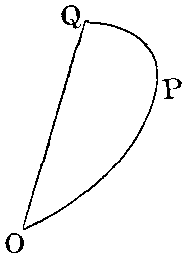
\includegraphics[width=20mm]{fig06.png}
\end{center}

\smallskip Composition of Successive Vectors.%
  \index{Composition!of successive components}%
  \index{Successive components!composition of}---The
composition of successive vectors partakes more of the nature of
multiplication than of addition. Let $A$ be a vector starting from
the point $O$, and $B$ a vector starting from the end of $A$. Draw
the third side $OP$, and from $O$ draw a vector equal to $B$, and
from its extremity a vector equal to $A$. The line $OP$ is not the
complete equivalent of $A + B$; if it were so, it would also be the
complete equivalent of $B + A$. But $A + B$ and $B + A$ determine
different paths; and as they go oppositely around, the areas they
determine with $OP$ have different signs. The diagonal $OP$
represents $A + B$ only so far as it is considered independent of
path. For any number of successive vectors, the sum so far as it is
independent of path is the vector from the initial point of the
first to the final point of the last. This is also true when the
successive vectors become so small as to form a continuous curve.
The area between the curve $OPQ$ and the vector $OQ$ depends on the
path, and has a physical meaning. \bigskip

\small \begin{enumerate}

\item[Prob.~1.] The resultant vector is $123\underline{/45^\circ}$,
and one component is $100\underline{/0^\circ}$; find the other
component.

\item[Prob.~2.] The velocity of a body in a given plane is
$200\underline{/75^\circ}$, and one component is
$100\underline{/25^\circ}$; find the other component.

\item[Prob.~3.] Three alternating magnetomotive forces are of equal
virtual value, but each pair differs in phase by $120^\circ$; find
the resultant. \hfill (Ans.~Zero.)

\item[Prob.~4.] Find the components of the vector
$100\underline{/70^\circ}$ in the directions $20^\circ$ and
$100^\circ$.

\item[Prob.~5.] Calculate the resultant vector of
$1\underline{/10^\circ}$, $2\underline{/20^\circ}$,
$3\underline{/30^\circ}$, $4\underline{/40^\circ}$.

\item[Prob.~6.] Compound the following magnetic fluxes: $h \sin nt + h
\sin (nt - 120^\circ)\underline{/120^\circ} + h \sin (nt -
240^\circ)\underline{/240^\circ}$. \hfill
(Ans.~$\frac{3}{2}h\underline{/nt}$.)

\item[Prob.~7.] Compound two alternating magnetic fluxes at a point $a
\cos nt \underline{/0}$ and $a \sin nt \underline{/\frac{\pi}{2}}$.
(Ans.~$a \underline{/nt}$.)

\item[Prob.~8.] Find the resultant of two simple alternating
electromotive forces $100\underline{/20^\circ}$ and
$50\underline{/75^\circ}$.

\item[Prob.~9.] Prove that a uniform circular motion is obtained by
compounding two equal simple harmonic motions which have the
space-phase of their angular positions equal to the supplement of
the time-phase of their motions.
\end{enumerate} \normalsize

\chapter{Products of Coplanar Vectors.}%
\index{Coplanar vectors}%
\index{Product!of two coplanar vectors}%
\index{Rules!for vectors}%
\index{Scalar product!of two coplanar vectors}%
\index{Vector!co-planar}

When all the vectors considered are confined to a common plane, each
may be expressed as the sum of two rectangular components. Let $i$
and $j$ denote two directions in the plane at right angles to one
another; then $A = a_1i + a_2j$, $B = b_1i + b_2j$, $R = xi + yj$.
Here $i$ and $j$ are not unit-vectors, but rather signs of
direction.

\smallskip Product of two Vectors.---Let $A = a_1i + a_2j$ and $B =
b_1i + b_2j$ be any two vectors, not necessarily of the same kind
physically. We assume that their product is obtained by applying the
distributive law, but we do not assume that the order of the factors
is indifferent. Hence
\begin{equation*}
AB = (a_1i + a_2j)(b_1i+b_2j) = a_1b_1ii + a_2b_2jj +
        a_1b_2ij + a_2b_2ji.
\end{equation*}

If we assume, as suggested by ordinary algebra, that the
square of a sign of direction is $+$, and further that the product
of two directions at right angles to one another is the direction
normal to both, then the above reduces to
\begin{equation*}
AB = a_1b_1 + a_2b_2 + (a_1b_2 - a_2b_1)k.
\end{equation*}

Thus the complete product%
\index{Complete product!of two vectors}%
\index{Product!complete} breaks up into two partial products%
\index{Partial products}%
\index{Product!partial}, namely, $a_1b_1 + a_2b_2$ which is
independent of direction, and $(a_1b_2 - a_2b_1)k$ which has the
axis of the plane for direction.\footnote{A common explanation which
is given of $ij = k$ is that $i$ is an operator, $j$ an operand, and
$k$ the result. The kind of operator which $i$ is supposed to denote
is a quadrant of turning round the axis $i$; it is supposed not to
be an axis, but a quadrant of rotation round an axis. This explains
the result $ij = k$, but unfortunately it does not explain $ii = +$;
for it would give $ii = i$.}

\begin{center}
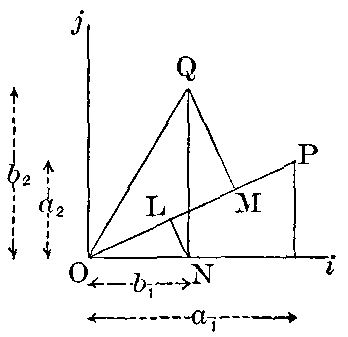
\includegraphics[width=40mm]{fig07.png}
\end{center}

\smallskip Scalar Product of two Vectors.%
\index{Product!scalar}%
\index{Scalar product}---By a scalar quantity is meant a quantity
which has magnitude and may be positive or negative but is destitute
of direction. The former partial product is so called because it is
of such a nature. It is denoted by $\mathrm{S}AB$ where the symbol
S, being in Roman type, denotes, not a vector, but a function of the
vectors $A$ and $B$.\index{Meaning!of S} The geometrical meaning of
$\mathrm{S}AB$ is the product of $A$ and the orthogonal projection
of $B$ upon $A$.\index{Scalar product!geometrical meaning} Let $OP$
and $OQ$ represent the vectors $A$ and $B$; draw $QM$ and $NL$
perpendicular to $OP$. Then
\begin{align*}
(OP)(OM) &= (OP)(OL) + (OP)(LM),  \\
         &= a\left\{ b_1\frac{a_1}{a} + b_2\frac{a_2}{a} \right\},  \\
         &= a_1b_1 + a_2b_2.
\end{align*}

\smallskip Corollary 1.---$\mathrm{S}BA = \mathrm{S}AB$. For instance,
let $A$ denote a force and $B$ the velocity of its point of
application; then $\mathrm{S}AB$ denotes the rate of working of the
force. The result is the same whether the force is projected on the
velocity or the velocity on the force.

\medskip Example 1.---A force of $2$ pounds East + $3$ pounds North
is moved with a velocity of $4$ feet East per second + $5$ feet
North per second; find the rate at which work is done.
\begin{equation*}
  2\times 4 + 3\times 5 = 23 \text{ foot-pounds per second.}
\end{equation*}

\smallskip Corollary 2.---$A^2 = a_1^2 + a_2^2 = a^2$. The square of
any vector is independent of direction;\index{Square!of a vector} it
is an essentially positive or signless quantity; for whatever the
direction of $A$, the direction of the other $A$ must be the same;
hence the scalar product cannot be negative.

\medskip Example 2.---A stone of $10$ pounds mass is moving with a
velocity $64$ feet down per second + $100$ feet horizontal per
second. Its kinetic energy then is
\begin{equation*}
  \frac{10}{2} (64^2 + 100^2) \text{ foot-poundals,}
\end{equation*}
a quantity which has no direction. The kinetic energy due to the
downward velocity is $10\times\dfrac{64^2}{2}$ and that due to the
horizontal velocity is $\dfrac{10}{2} \times 100^2$; the whole
kinetic energy is obtained, not by vector, but by simple addition,
when the components are rectangular.

\begin{center}
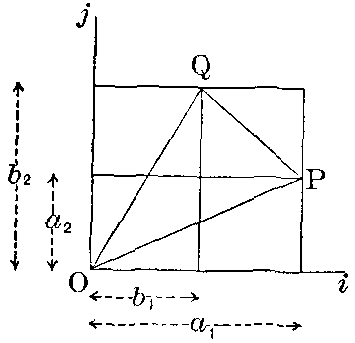
\includegraphics[width=40mm]{fig08.png}
\end{center}

\smallskip Vector Product of two Vectors.%
\index{Product!vector}%
\index{Vector product}%
\index{Vector product!of two vectors}---The other partial product
from its nature is called the vector product, and is denoted by
$\mathrm{V}AB$.\index{Meaning!of V} Its geometrical meaning is the
product of $A$ and the projection of $B$ which is perpendicular to
$A$, that is, the area of the parallelogram formed upon $A$ and $B$.
Let $OP$ and $OQ$ represent the vectors $A$ and $B$, and draw the
lines indicated by the figure. It is then evident that the area of
the triangle $OPQ = a_1 b_2 - \frac{1}{2} a_2 a_2 - \frac{1}{2} b_1
b_2 - \frac{1}{2} (a_1 - b_1)(b_2 - a_2) = \frac{1}{2}(a_1 b_2 - a_2
b_1)$.

Thus $(a_1 b_2 - a_2 b_1)k$ denotes the magnitude of the
parallelogram formed by $A$ and $B$ and also the axis of the plane
in which it lies.

It follows that $\mathrm{V}BA = -\mathrm{V}AB$. It is to be observed
that the coordinates of $A$ and $B$ are mere component vectors,
whereas $A$ and $B$ themselves are taken in a real order.

\medskip Example.---Let $A = (10i + 11j)$~inches and $B = (5i +
12j)$~inches, then $\mathrm{V}AB = (120-55)k$~square inches; that
is, 65~square inches in the plane which has the direction $k$ for
axis.

\medskip If $A$ is expressed as $a\alpha$ and $B$ as $b\beta$, then
$\mathrm{S}AB = ab \cos \alpha\beta$, where $\alpha\beta$ denotes
the angle between the directions $\alpha$ and $\beta$.

\medskip Example.---The effective electromotive force of $100$~volts
per inch $\underline{/90^\circ}$ along a conductor $8$~inch
$\underline{/45^\circ}$ is $\mathrm{S}AB = 8 \times 100\,
\cos\underline{/45^\circ}\underline{/90^\circ}$~volts, that is, $800
\cos 45^\circ$ volts. Here $\underline{/45^\circ}$ indicates the
direction $\alpha$ and $\underline{/90^\circ}$ the direction
$\beta$, and $\underline{/45^\circ}\underline{/90^\circ}$ means the
angle between the direction of $45^\circ$ and the direction of
$90^\circ$.

\smallskip Also $\mathrm{V}AB = ab \sin \alpha\beta \cdot
\overline{\alpha\beta}$, where $\overline{\alpha\beta}$ denotes the
direction which is normal to both $\alpha$ and $\beta$, that is,
their pole.\index{Meaning!of vinculum over two axes}

\smallskip Example.---At a distance of $10$ feet
$\underline{/30^\circ}$ there is a force of $100$ pounds
$\underline{/60^\circ}$ The moment is $\mathrm{V}AB$
\begin{align*}
&= 10 \times 100 \sin \underline{/30^\circ} \underline{/60^\circ}
  \text{ pound-feet } \overline{90^\circ/}\underline{/90^\circ} \\
&= 1000 \sin 30^\circ \text{ pound feet }
  \overline{90^\circ/}\underline{/90^\circ}
\end{align*}

Here $\overline{90^\circ/}$ specifies the plane of the angle and
$\underline{/90^\circ}$ the angle. The two together written as above
specify the normal $k$.

\medskip Reciprocal of a Vector.%
\index{Reciprocal!of a vector}%
\index{Vector!reciprocal of}---By the reciprocal of a vector is
meant the vector which combined with the original vector produces
the product $+1$. The reciprocal of $A$ is denoted by $A^{-1}$.
Since $AB = ab (\cos \alpha\beta + \sin \alpha\beta \cdot
\overline{\alpha\beta})$, $b$ must equal $a^{-1}$ and $\beta$ must
be identical with $\alpha$ in order that the product may be $1$. It
follows that
\begin{equation*}
A^{-1} = \frac{1}{a}\alpha = \frac{a\alpha}{a^2} = \frac{a_1i +
a_2j}{a_1^2 + a_2^2}.
\end{equation*}

\begin{center}
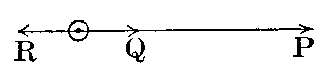
\includegraphics[width=40mm]{fig09.png}
\end{center}

The reciprocal and opposite vector is $-A^{-1}$.%
\index{Opposite vector}%
\index{Vector!opposite of} In the figure let $OP = 2\beta$ be the
given vector; then $OQ = \frac{1}{2}\beta$ is its reciprocal, and
$OR =\frac{1}{2}(-\beta)$ is its reciprocal and
opposite.\footnote{Writers who identify a vector with a quadrantal
versor\index{Quadrantal versor} are logically led to define the
reciprocal of a vector as being opposite in direction as well as
reciprocal in magnitude.}

\smallskip Example.---If $A = 10 \text{ feet East} + 5 \text{ feet
North}$, $A^{-1}= \dfrac{10}{125} \text{ feet East} \ +$ \\
$\dfrac{5}{125} \text{ feet North}$ and $-A^{-1}=-\dfrac{10}{125}
\text{ feet East} - \dfrac{5}{125}\text{ feet North}$.

\smallskip Product of the reciprocal of a vector and another
vector.---
\begin{align*}
A^{-1}B &= \frac{1}{a^2}AB, \\
  &= \frac{1}{a^2}\left\{a_1b_1 + a_2b_2 + (a_1b_2 - a_2b_1)
       \overline{\alpha\beta}\right\}, \\
  &= \frac{b}{a}(\cos \alpha\beta + \sin\alpha\beta \cdot
       \overline{\alpha\beta}).
\end{align*}

Hence $\mathrm{S}A^{-1}B = \dfrac{b}{a}\cos \alpha\beta$ and
$\mathrm{V}A^{-1}B = \dfrac{b}{a} \sin \alpha\beta \cdot
\overline{\alpha\beta}$.

\newpage
\medskip Product of three Coplanar Vectors.%
\index{Association of three vectors}%
\index{Product!of three coplanar vectors}---Let $A = a_1i + a_2j$,
$B = b_1i + b_2j$, $C = c_1i + c_2j$ denote any three vectors in a
common plane. Then
\begin{align*}
(AB)C &= \bigl\{(a_1b_1 + a_2b_2) + (a_1b_2 - a_2b_1)k \bigr\}
            (c_1i + c_2j) \\
      &= (a_1b_1 + a_2b_2)(c_1i + c_2j) +
            (a_1b_2 - a_2b_1)(-c_2i + c_1j).
\end{align*}

\begin{center}
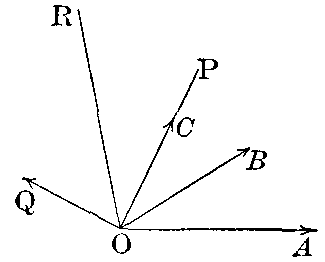
\includegraphics[width=40mm]{fig10.png}
\end{center}

The former partial product means the vector $C$ multiplied by the
scalar product of $A$ and $B$; while the latter partial product
means the complementary vector of $C$ multiplied by the magnitude of
the vector product of $A$ and $B$. If these partial products
(represented by $OP$ and $OQ$) unite to form a total product, the
total product will be represented by $OR$, the resultant of $OP$ and
$OQ$.

The former product is also expressed by $\mathrm{S}AB \cdot C$,
where the point separates the vectors to which the $\mathrm{S}$
refers; and more analytically by $abc \cos \alpha\beta \cdot
\gamma$.

The latter product is also expressed by $(\mathrm{V}AB)C$, which is
equivalent to $\mathrm{V}(\mathrm{V}AB)C$, because $\mathrm{V}AB$ is
at right angles to $C$. It is also expressed by $abc \sin
\alpha\beta \cdot \overline{\overline{\alpha\beta}\gamma}$, where
$\overline{\overline{\alpha\beta}\gamma}$ denotes the direction
which is perpendicular to the perpendicular to $\alpha$ and $\beta$
and $\gamma$.

If the product is formed after the other mode of association
we have
\begin{align*}
A(BC) &= (a_1i + a_2j)(b_1c_1 + b_2c_2) +
           (a_1i + a_2j)(b_1c_2 - b_2c_1)k \\
      &= (b_1c_1 + b_2c_2)(a_1i + a_2j) +
           (b_1c_2 - b_2c_1)(a_2i - a_1j) \\
      &= \mathrm{S}BC \cdot A + \mathrm{V}A(\mathrm{V}BC).
\end{align*}

The vector $a_2i - a_1j$ is the opposite of the complementary
vector of $a_1i + a_2j$. Hence the latter partial product differs
with the mode of association.

\smallskip Example.---Let $A = 1\underline{/0^\circ} +
2\underline{/90^\circ}$, $B = 3\underline{/0^\circ} +
4\underline{/90^\circ}$, $C = 5\underline{/0^\circ} +
6\underline{/90^\circ}$. The fourth proportional to $A, B, C$ is
\begin{align*}
(A^{-1}B)C &=
   \frac{1 \times 3 + 2 \times 4}{1^2 + 2^2}
   \left\{ 5 \underline{/0^\circ}
         + 6 \underline{/90^\circ}\right\} \\
&\quad + \frac{1 \times 4 - 2 \times 3}{1^2 + 2^2}
     \left\{ -6 \underline{/0^\circ} +
                                  5 \underline{/90^\circ}\right \} \\
&= 13.4 \underline{/0^\circ} + 11.2 \underline{/90^\circ}.
\end{align*}

\medskip Square of a Binomial of Vectors.%
\index{Square!of two simultaneous components}---If $A + B$
denotes a sum of non-successive vectors, it is entirely equivalent
to the resultant vector $C$. But the square of any vector is a
positive scalar, hence the square of $A + B$ must be a positive
scalar. Since $A$ and $B$ are in reality components of one vector,
the square must be formed after the rules for the products of
rectangular components (p.\ 432). Hence
\begin{align*}
(A + B)^2 &= (A + B)(A + B), \\
          &= A^2 + AB + BA + B^2, \\
          &= A^2 + B^2 + \mathrm{S}AB + \mathrm{S}BA +
               \mathrm{V}AB + \mathrm{V}BA, \\
          &= A^2 + B^2 + 2\mathrm{S}AB.
\end{align*}
This may also be written in the form
\begin{equation*}
a^2 + b^2 + 2ab\cos\alpha\beta.
\end{equation*}

But when $A + B$ denotes a sum of successive vectors, there is no
third vector $C$ which is the complete equivalent; and consequently
we need not expect the square to be a scalar quantity.%
\index{Square!of two successive components} We observe that there is
a real order, not of the factors, but of the terms in the binomial;
this causes both product terms to be $AB$, giving
\begin{align*}
(A + B)^2 &=  A^2 + 2AB + B^2 \\
          &=  A^2+B^2 + 2\mathrm{S}AB + 2\mathrm{V}AB.
\end{align*}

The scalar part gives the square of the length of the third
side, while the vector part gives four times the area included
between the path and the third side.

\smallskip Square of a Trinomial of Coplanar Vectors.%
\index{Square!of three successive components}---Let $A + B + C$
denote a sum of successive vectors. The product terms must be formed
so as to preserve the order of the vectors in the trinomial; that
is, $A$ is prior to $B$ and $C$, and $B$ is prior to $C$. Hence
\begin{align}
(A + B + C)^2 &= A^2 + B^2 + C^2 + 2AB + 2AC + 2BC, \notag \\
              &= A^2 + B^2 + C^2 + 2(\mathrm{S}AB +
                  \mathrm{S}AC + \mathrm{S}BC), \tag{1} \\
              &\qquad + 2(\mathrm{V}AB + \mathrm{V}AC +
                  \mathrm{V}BC). \tag{2}
\end{align}
Hence
\begin{gather*}
\mathrm{S}(A+B+C)^2 = (1) \\
= a^2 + b^2 + c^2 + 2ab\cos \alpha\beta
  + 2ac\cos \alpha\gamma + 2bc\cos\beta\gamma \\
\intertext{and}
\mathrm{V}(A+B+C)^2 = (2) \\
= \{ 2ab\sin\alpha\beta + 2ac\sin\alpha\gamma + 2bc\sin\beta\gamma\}
  \cdot \overline{\alpha\beta}
\end{gather*}

\begin{center}
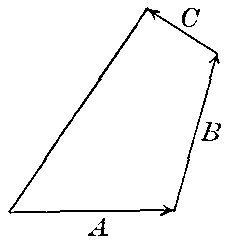
\includegraphics[width=35mm]{fig11.png}
\end{center}

The scalar part gives the square of the vector from the beginning of
$A$ to the end of $C$ and is all that exists when the vectors are
non-successive. The vector part is four times the area included
between the successive sides and the resultant side of the polygon.

Note that it is here assumed that $\mathrm{V}(A + B)C = \mathrm{V}AC
+ \mathrm{V}BC$, which is the theorem of moments. Also that the
product terms are not formed in cyclical order, but in accordance
with the order of the vectors in the trinomial.%
\index{Cyclical and natural order}%
\index{Natural order}

\smallskip Example.---Let $A = 3\underline{/0^\circ}$,
$B = 5\underline{/30^\circ}$, $C = 7\underline{/45^\circ}$; find the
area of the polygon.
\begin{align*}
\frac{1}{2}\mathrm{V}(AB + AC + BC) &=
\frac{1}{2}\{15\sin\underline{/0^\circ}\underline{/30^\circ} +
        21\sin\underline{/0^\circ}\underline{/45^\circ} +
        35\underline{/30^\circ}\underline{/45^\circ}\}, \\
&= 3.75 + 7.42 + 4.53 = 15.7.
\end{align*}

\small \begin{enumerate}
\item[Prob.~10.] At a distance of $25$ centimeters
$\underline{/20^\circ}$ there is a force of 1000~dynes
$\underline{/80^\circ}$; find the moment.

\item[Prob.~11.] A conductor in an armature has a velocity of
240~inches per second $\underline{/300^\circ}$ and the magnetic flux
is 50,000~lines per square inch $\underline{/0^\circ}$; find the
vector product. (Ans.~$1.04 \times 10^7$~lines per inch per second.)

\item[Prob.~12.] Find the sine and cosine of the angle between the
directions 0.8141~E.\ + 0.5807~N., and 0.5060~E.\ + 0.8625~N.

\item[Prob.~13.] When a force of 200~pounds $\underline{/270^\circ}$ is
displaced by 10~feet $\underline{/30^\circ}$, what is the work done
(scalar product)? What is the meaning of the negative sign in the
scalar product?

\item[Prob.~14.] A mass of $100$ pounds is moving with a velocity of
30 feet E.\ per second + 50 feet SE.\ per second; find its kinetic
energy.

\item[Prob.~15.] A force of $10$ pounds $\underline{/45^\circ}$ is
acting at the end of $8$ feet $\underline{/200^\circ}$; find the
torque, or vector product.

\item[Prob.~16.] The radius of curvature of a curve is
$2\underline{/0^\circ} + 5\underline{/90^\circ}$; find the
curvature. \\ (Ans.~$.03\underline{/0^\circ} +
.17\underline{/90^\circ}$.)

\item[Prob.~17.] Find the fourth proportional to
$10\underline{/0^\circ} + 2\underline{/90^\circ}$,
$8\underline{/0^\circ} - 3\underline{/90^\circ}$, and
$6\underline{/0^\circ} + 5\underline{/90^\circ}$.

\item[Prob.~18.] Find the area of the polygon whose successive sides
are $10\underline{/30^\circ}$, $9\underline{/100^\circ}$,
$8\underline{/180^\circ}$, $7\underline{/225^\circ}$.
\end{enumerate} \normalsize

\chapter{Coaxial Quaternions.}%
\index{Coaxial Quaternions}%
\index{Quaternions!Coaxial}

By a ``quaternion'' is meant the operator which changes one vector
into another. It is composed of a magnitude and a turning factor.%
\index{Components!of versor}%
\index{Quaternion!definition of}%
\index{Versor!components of} The magnitude may or may not be a mere
ratio, that is, a quantity destitute of physical dimensions; for the
two vectors may or may not be of the same physical kind. The turning
is in a plane, that is to say, it is not conical. For the present
all the vectors considered lie in a common plane; hence all the
quaternions considered have a common axis.\footnote{The idea of the
``quaternion'' is due to Hamilton.\index{Hamilton's!idea of
quaternion} Its importance may be judged from the fact that it has
made solid trigonometrical analysis possible. It is the most
important key to the extension of analysis to space. Etymologically
``quaternion'' means defined by four elements; which is true in
space; in plane analysis it is defined by two.%
\index{Quaternion!etymology of}}

\begin{center}
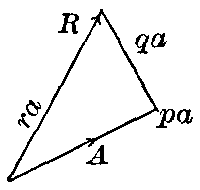
\includegraphics[width=30mm]{fig12.png}
\end{center}

Let $A$ and $R$ be two coinitial vectors; the direction normal to
the plane may be denoted by $\beta$. The operator which changes $A$
into $R$ consists of a scalar multiplier and a turning round the
axis $\beta$. Let the former be denoted by $r$ and the latter by
$\beta^\theta$, where $\theta$ denotes the angle in radians. Thus $R
= r\beta^\theta A$ and reciprocally $A =
\dfrac{1}{r}\beta^{-\theta}R$. Also $\dfrac{1}{A}R = r\beta^\theta$
and $\dfrac{1}{R}A = \dfrac{1}{r}\beta^{-\theta}$.

The turning factor $\beta^\theta$ may be expressed as the sum of two
component operators, one of which has a zero angle and the other an
angle of a quadrant. Thus
\begin{equation*}
\beta^\theta = \cos\theta \cdot \beta^\theta + \sin\theta \cdot
\beta^\frac{\pi}{2}.
\end{equation*}

When the angle is naught, the turning-factor may be omitted; but the
above form shows that the equation is homogeneous, and expresses
nothing but the equivalence of a given quaternion to two component
quaternions.\footnote{In the method of complex numbers
$\beta^\frac{\pi}{2}$ is expressed by $i$, which stands for
$\sqrt{-1}$.%
\index{Algebraic imaginary}%
\index{Imaginary algebraic} The advantages of using the above
notation are that it is capable of being applied to space, and that
it also serves to specify the general turning factor $\beta^\theta$
as well as the quadrantal turning factor
$\beta^\frac{\pi}{2}$.}\index{Components!of quaternion}

Hence
\begin{align*}
r\beta^\theta & = r\cos\theta +
                             r\sin\theta \cdot \beta^\frac{\pi}{2} \\
& = p + q \cdot \beta^\frac{\pi}{2} \\
\intertext{and}
r\beta^\theta A & = pA + q \beta^\frac{\pi}{2} A \\
& = pa \cdot \alpha + qa \cdot \beta^\frac{\pi}{2} \alpha.
\end{align*}

The relations between $r$ and $\theta$, and $p$ and $q$, are given by
\begin{equation*}
r = \sqrt{p^2 + q^2}, \quad \theta = \tan^{-1} \frac{p}{q}.
\end{equation*}

\medskip Example.---Let $E$ denote a sine alternating electromotive
force in magnitude and phase, and $I$ the alternating current in
magnitude and phase, then
\begin{equation*}
E = \left(r + 2\pi n l \cdot \beta^\frac{\pi}{2} \right) I,
\end{equation*}
where $r$ is the resistance, $l$ the self-induction, $n$ the
alternations per unit of time, and $\beta$ denotes the axis of the
plane of representation. It follows that $E = rI + 2\pi n l \cdot
\beta^\frac{\pi}{2} I$; also that
\begin{equation*}
I^{-1} E = r + 2\pi n l \cdot \beta^\frac{\pi}{2},
\end{equation*}
that is, the operator which changes the current into the
electromotive force is a quaternion. The resistance is the scalar
part of the quaternion, and the inductance is the vector part.

\medskip Components of the Reciprocal of a Quaternion.%
\index{Components!of reciprocal of quaternion}%
\index{Quaternion!reciprocal of}%
\index{Reciprocal!of a quaternion}---Given
\begin{equation*}
R = \left(p + q \cdot \beta^\frac{\pi}{2} \right) A,
\end{equation*}
then
\begin{align*}
A & = \frac{1}{p + q \cdot \beta^\frac{\pi}{2}} R \\
  & = \frac{p - q \cdot \beta^\frac{\pi}{2}}
                       {\left(p + q \cdot \beta^\frac{\pi}{2} \right)
      \left(p - q \cdot \beta^\frac{\pi}{2} \right)} R \\
  & = \frac{p - q \cdot \beta^\frac{\pi}{2}}{p^2 + q^2} R \\
  & = \left\{ \frac{p}{p^2 + q^2} - \frac{q}{p^2 + q^2} \cdot
    \beta^\frac{\pi}{2} \right\} R.
\end{align*}

\smallskip Example.---Take the same application as above. It is
important to obtain $I$ in terms of $E$. By the above we deduce that
from $E = (r + 2\pi nl \cdot \beta^\frac{\pi}{2})I$
\begin{equation*}
I = \left\{\frac{r}{r^2+(2\pi nl)^2} -
  \frac{2\pi nl}{r^2+(2\pi nl)^2}\cdot \beta^\frac{\pi}{2}\right\}E.
\end{equation*}

\medskip Addition of Coaxial Quaternions.%
\index{Coaxial Quaternions!Addition of}---If the ratio of each of
several vectors to a constant vector $A$ is given, the ratio of
their resultant to the same constant vector is obtained by taking
the sum of the ratios. Thus, if
\begin{align*}
R_1 &= (p_1 + q_1 \cdot \beta^\frac{\pi}{2}) A, \\
R_2 &= (p_2 + q_2 \cdot \beta^\frac{\pi}{2}) A, \\
\qquad \qquad \vdots & \qquad \vdots \qquad \vdots \qquad \vdots \\
R_n &= (p_n + q_n \cdot \beta^\frac{\pi}{2}) A, \\
\intertext{then}
\sum R &= \left\{\sum p + \left(\sum q\right) \cdot
                                   \beta^\frac{\pi}{2}\right\}A, \\
\intertext{and reciprocally}
A &= \frac{\sum p - \left(\sum q \right) \cdot \beta^\frac{\pi}{2}}
          {\left( \sum p\ \right)^2 + \left( \sum q \right)^2}\sum R.
\end{align*}

\smallskip Example.\index{Composition!of coaxial quaternions}---In
the case of a compound circuit composed of a number of simple
circuits in parallel
\begin{equation*}
I_1 = \frac{r_1 - 2\pi nl_1 \cdot
  \beta^\frac{\pi}{2}}{r_1^2 + (2\pi n)^2 l_1^2}E, \quad
I_2 = \frac{r_2 - 2\pi nl_2 \cdot \beta^\frac{\pi}{2}}{r_2^2 +
  (2\pi n)^2 l_2^2}E, \quad \text{etc.},
\end{equation*}
therefore,
\begin{align*}
\sum I & = \sum\left\{\frac{r - 2\pi nl \cdot
   \beta^\frac{\pi}{2}} {r^2 + (2\pi n)^2 l^2}\right\}E \\
& = \left\{\sum\left(\frac{r}{r^2 + (2\pi n)^2l^2}\right) -
   2\pi n\sum\frac{l}{r^2 + (2\pi n)^2l^2} \cdot
   \beta^\frac{\pi}{2}\right\}E,
\end{align*}
and reciprocally
\begin{equation*}
E = \frac{ \sum\left(\frac{r}{r^2 + (2\pi n)^2 l^2}\right) +
    2\pi n\sum\left(\frac{l}{r^2 + (2\pi n)^2 l^2}\right) \cdot
    \beta^\frac{\pi}{2}}
{\left(\sum\frac{r}{r^2 + (2\pi n)^2 l^2}\right)^2 +
    (2\pi n)^2\left(\sum\frac{l}{r^2 + (2\pi n)^2 l^2}\right)^2}
    \sum I.\footnotemark
\end{equation*}
\footnotetext{This theorem was discovered by Lord
Rayleigh\index{Rayleigh}; Philosophical Magazine, May, 1886. See
also Bedell \& Crehore's Alternating Currents, p.\ 238.}

\smallskip Product of Coaxial Quaternions.%
\index{Coaxial Quaternions!Product of}%
\index{Product!of coaxial quaternions}---If the quaternions which
change $A$ to $R$, and $R$ to $R'$, are given, the quaternion which
changes $A$ to $R'$ is obtained by taking the product of the given
quaternions.

Given
\begin{align*}
R  & = r\beta^\theta A = \left(p + q \cdot
                                       \beta^\frac{\pi}{2}\right)A \\
\intertext{and}
R' & = r'\beta^{\theta'}A = \left(p' +
                             q' \cdot \beta^\frac{\pi}{2}\right)R, \\
\intertext{then}
R' & = rr'\beta^{\theta+\theta'}A =
  \left\{(pp'-qq') + (pq'+p'q) \cdot \beta^\frac{\pi}{2}\right\}A.
\end{align*}

Note that the product is formed by taking the product of the
magnitudes, and likewise the product of the turning factors. The
angles are summed because they are indices of the common base
$\beta$.\footnote{Many writers, such as Hayward in ``Vector Algebra
and Trigonometry,'' and Stringham in ``Uniplanar Algebra,'' treat
this product of coaxial quaternions as if it were the product of
vectors.\index{Hayward}\index{Stringham} This is the fundamental
error in the Argand method.\index{Argand method}}

\smallskip Quotient of two Coaxial Quaternions.%
\index{Coaxial Quaternions!Quotient of}%
\index{Quotient of two coaxial quaternions}---If the given
quaternions are those which change $A$ to $R$, and $A$ to $R'$, then
that which changes $R$ to $R'$ is obtained by taking the quotient of
the latter by the former.

Given
\begin{align*}
R & = r\beta^\theta A = (p + q \cdot \beta^\frac{\pi}{2})A \\
\intertext{and}
R' & = r'\beta'^{\theta'} A = (p' + q' \cdot \beta^\frac{\pi}{2})A,\\
\intertext{then}
R' & = \frac{r'}{r}\beta^{\theta' - \theta}R, \\
   & = (p' + q' \cdot \beta^\frac{\pi}{2})\frac{1}{p + q \cdot
       \beta^\frac{\pi}{2}}R, \\
   & = (p' + q' \cdot \beta^\frac{\pi}{2})\frac{p - q \cdot
       \beta^\frac{\pi}{2}}{p^2 + q^2}R, \\
   & = \frac{(pp' + qq') + (pq' - p'q) \cdot
       \beta^\frac{\pi}{2}}{p^2 + q^2}R.
\end{align*}

\small \begin{enumerate}
\item[Prob.~19.] The impressed alternating electromotive force is
$200$ volts, the resistance of the circuit is $10$ ohms, the
self-induction is $\frac{1}{100}$ henry, and there are $60$
alternations per second; required the current. \hfill (Ans. $18.7$
amperes $\underline{/-20^\circ\,42'}$.)

\item[Prob.~20.] If in the above circuit the current is $10$
amperes, find the impressed voltage.

\item[Prob.~21.] If the electromotive force is $110$ volts
$\underline{/\theta}$ and the current is $10$ amperes
$\underline{/\theta - \frac{1}{4}\pi}$, find the resistance and the
self-induction, there being $120$ alternations per second.

\item[Prob.~22.] A number of coils having resistances $r_1$, $r_2$,
etc., and self-inductions $l_1$, $l_2$, etc., are placed in series;
find the impressed electromotive force in terms of the current, and
reciprocally.
\end{enumerate} \normalsize

\chapter{Addition of Vectors in Space.}

A vector in space can be expressed in terms of three independent
components, and when these form a rectangular set the directions of
resolution are expressed by $i$, $j$, $k$.%
\index{Composition!of simultaneous vectors in space}%
\index{Vector!in space} Any variable vector $R$ may be expressed as
$R = r\rho = xi + yj + zk$, and any constant vector $B$ may be
expressed as
\begin{equation*}
B = b\beta = b_1i + b_2j + b_3k.
\end{equation*}

In space the symbol $\rho$ for the direction involves two elements.
It may be specified as
\begin{equation*}
\rho = \frac{xi + yj + zk}{x^2 + y^2 + z^2},
\end{equation*}
where the three squares are subject to the condition that their sum
is unity. Or it may be specified by this notation,
$\overline{\phi/}\!\underline{/\theta}$, a generalization of the
notation for a plane.\index{Meaning!of $\overline{\ /}$} The
additional angle $\overline{\phi/}$ is introduced to specify the
plane in which the angle from the initial line lies.

If we are given $R$ in the form $r\overline{\phi/}\!
\underline{/\theta}$, then we deduce the other form thus:
\begin{equation*}
R = r \cos\theta \cdot i + r \sin\theta \cos \phi \cdot j
    + r \sin\theta \sin\phi \cdot k.
\end{equation*}

If $R$ is given in the form $xi + yj + zk$, we deduce
\begin{gather*}
R = \sqrt{x^2 + y^2 + z^2}\
\overline{\left.\tan^{-1}\frac{z}{y}\right/}\!\!\!\!
\underline{\left/\tan^{-1}\frac{\sqrt{y^2 + z^2}}{x}\right.}. \\
\intertext{For example,}
\begin{aligned}
B &= 10\ \overline{30^\circ/}\! \underline{/45^\circ} \\
  &= 10 \cos 45^\circ \cdot i
     + 10 \sin 45^\circ \cos 30^\circ \cdot j
     + 10 \sin 45^\circ \sin 30^\circ \cdot k.
\end{aligned}
\end{gather*}

Again, from $C = 3i + 4j + 5k$ we deduce
\begin{align*}
C & = \sqrt{9 + 16 + 25}\
      \overline{\left.\tan^{-1}\frac{5}{4}\right/}\!\!\!\!
      \underline{\left/\tan^{-1}\frac{\sqrt{41}}{3}\right.} \\
  & = 7.07\ \overline{51^\circ.4/}\! \underline{/64^\circ.9}.
\end{align*}

To find the resultant of any number of component vectors applied at
a common point, let $R_1$, $R_2$, $\ldots$ $R_n$ represent the $n$
vectors or,
\begin{align*}
R_1 &= x_1i + y_1j + z_1k, \\
R_2 &= x_2i + y_2j + z_2k, \\
\cdots & \cdots\cdots\cdots\cdots\cdots\cdots \\
R_n &= x_ni + y_nj + z_nk; \\
\intertext{then}
\sum R &= \left(\sum x \right)i + \left(\sum y \right)j +
  \left(\sum z \right)k \\
\intertext{and}
r &= \sqrt{\left(\sum x \right)^2 + \left(\sum y \right)^2 +
  \left(\sum z \right)^2}, \\
\tan\phi &= \frac{\sum z}{\sum y} \text{ and }
  \tan\theta = \frac{\sqrt{\left(\sum y \right)^2
         + \left(\sum z \right)^2}}{\sum x}.
\end{align*}

\medskip Successive Addition.---When the successive vectors do not
lie in one plane, the several elements of the area enclosed will lie
in different planes, but these add by vector addition into a
resultant directed area.

\small \begin{enumerate}
\item[Prob.~23.] Express $A = 4i - 5j + 6k$ and $B = 5i + 6j - 7k$ in
the form $r\overline{\phi/}\!\underline{/\theta}$ \\ (Ans.~$8.8\
\overline{130^\circ/}\!\underline{/63^\circ}$ and $10.5\
\overline{311^\circ/}\!\underline{/61^\circ .5}$.)

\item[Prob.~24.] Express $C = 123\
\overline{57^\circ/}\!\underline{/142^\circ}$ and $D = 456\
\overline{65^\circ/}\!\underline{/200^\circ}$ in the form $xi + yj +
zk$.

\item[Prob.~25.] Express $E =
100\ \overline{\left.\dfrac{\pi}{4}\right/}\!\!\!
\underline{\left/\dfrac{\pi}{3}\right.}$ and $F = 1000\
\overline{\left.\dfrac{\pi}{6}\right/}\!\!\!\underline{\left/
\dfrac{3\pi}{4}\right.}$ in the form $xi + yj + zk$.

\item[Prob.~26.] Find the resultant of $10\ \overline{20^\circ /}\!
\underline{/30^\circ}$, $20\ \overline{30^\circ /}\!
\underline{/40^\circ}$, and $30\ \overline{40^\circ /}\!
\underline{/50^\circ}$.

\item[Prob.~27.] Express in the form $r\ \overline{\phi/}\!
\underline{/\theta}$ the resultant vector of $1i + 2j - 3k$, $4i -
5j + 6k$ and $-7i + 8j + 9k$.
\end{enumerate} \normalsize

\chapter{Product of Two Vectors.}

Rules of Signs for Vectors in Space.\index{Rules!for vectors}---By
the rules $i^2 =+$, $j^2 = +$, $ij = k$, and $ji =-k$ we obtained
(p.\ 432) a product of two vectors containing two partial products,
each of which has the highest importance in mathematical and
physical analysis. Accordingly, from the symmetry of space we assume
that the following rules are true for the product of two vectors in
space:
\begin{align*}
i^2 &=  +, & j^2 &=  +, & k^2 &=  + \, , \\
ij  &=  k, & jk  &=  i, & ki  &=  j \, , \\
ji  &= -k, & kj  &= -i, & ik  &= -j \, .
\end{align*}

\begin{center}
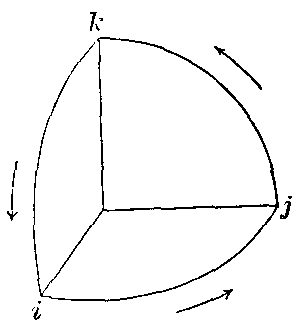
\includegraphics[width=30mm]{fig13.png}
\end{center}

The square combinations give results which are independent of
direction, and consequently are summed by simple addition. The area
vector determined by $i$ and $j$ can be represented in direction by
$k$, because $k$ is in tri-dimensional space the axis which is
complementary to $i$ and $j$. We also observe that the three rules
$ij = k$, $jk = i$, $ki = j$ are derived from one another by
cyclical permutation; likewise the three rules $ji = -k$, $kj = -i$,
$ik = -j$. The figure shows that these rules are made to represent
the relation of the advance to the rotation in the right-handed
screw. The physical meaning of these rules is made clearer by an
application to the dynamo and the electric motor. In the dynamo
three principal vectors have to be considered: the velocity of the
conductor at any instant, the intensity of magnetic flux, and the
vector of electromotive force. Frequently all that is demanded is,
given two of these directions to determine the third. Suppose that
the direction of the velocity is $i$, and that of the flux $j$, then
the direction of the electromotive force is $k$. The formula $ij =
k$ becomes
\begin{gather*}
\text{velocity flux} = \text{electromotive-force},\\
\intertext{from which we deduce}
\text{flux electromotive-force} = \text{velocity}, \\
\intertext{and}
\text{electromotive-force velocity} = \text{flux}.
\end{gather*}

The corresponding formula for the electric motor is %
\index{Dynamo rule}%
\index{Electric motor rule}%
\index{Rules!for dynamo}
\begin{equation*}
\text{current flux} = \text{mechanical-force},
\end{equation*}
from which we derive by cyclical permutation
\begin{equation*}
   \text{flux force} = \text{current},
\quad\text{and}\quad
   \text{force current} = \text{flux}.
\end{equation*}

The formula $\text{velocity flux} = \text{electromotive-force}$ is much
handier than any thumb-and-finger rule; for it compares the
three directions directly with the right-handed screw.

\medskip Example.---Suppose that the conductor is normal to the plane
of the paper, that its velocity is towards the bottom, and that the
magnetic flux is towards the left; corresponding to the rotation
from the velocity to the flux in the right-handed screw we have
advance into the paper: that then is the direction of the
electromotive force.%
\index{Relation of right-handed screw}%
\index{Screw, relation of right-handed}

Again, suppose that in a motor the direction of the current along
the conductor is up from the paper, and that the magnetic flux is to
the left; corresponding to current flux we have advance towards the
bottom of the page, which therefore must be the direction of the
mechanical force which is applied to the conductor.

\medskip Complete Product of two Vectors%
\index{Complete product!of two vectors}%
\index{Product!complete}.---Let $A = a_1i + a_2j + a_3k$ and
$B = b_1i + b_2j + b_3k$ be any two vectors, not necessarily of the
same kind physically, Their product, according to the rules
(p.~444), is
\begin{align*}
AB &= (a_1i + a_2j + a_3k)(b_1i + b_2j + b_3k), \\
   &= a_1 b_1 ii + a_2 b_2 jj + a_3 b_3 kk \\
   & \qquad + a_2 b_3 jk + a_3 b_2 kj + a_3 b_1 ki + a_1 b_3 ik
     + a_1 b_2 ij + a_2 b_1 ji \\
   &= a_1 b_1 + a_2 b_2 + a_3 b_3 \\
   & \qquad + (a_2 b_3)i + (a_3 b_1 - a_1 b_3)j
     + (a_1 b_2 - a_2 b_1)k \\
   &= a_1 b_1 + a_2 b_2 +a_3 b_3 +
            \begin{vmatrix}
               a_1 & a_2 & a_3 \\
               b_1 & b_2 & b_3 \\
               i   & j   & k
            \end{vmatrix}
\end{align*}

Thus the product breaks up into two partial products%
\index{Partial products}%
\index{Product!partial}, namely, $a_1 b_1 + a_2 b_2 + a_3 b_3$,
which is independent of direction, and
$\begin{vmatrix} a_1 & a_2 & a_3 \\
                 b_1 & b_2 & b_3 \\
                 i   & j   & k
\end{vmatrix}$, which has the direction normal to the plane of
$A$ and $B$. The former is called the scalar product, and the latter
the vector product.%
\index{Determinant!for vector product of two vectors}

\smallskip In a sum of vectors, the vectors are necessarily
homogeneous, but in a product the vectors may be heterogeneous. By
making $a_3 = b_3 = 0$, we deduce the results already obtained for a
plane.

\begin{center}
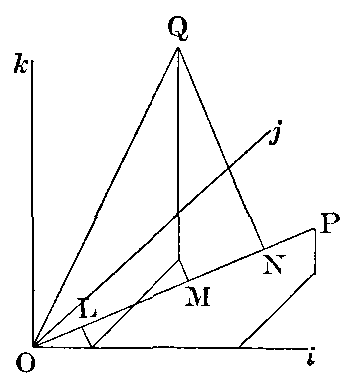
\includegraphics[width=30mm]{fig14.png}
\end{center}

\smallskip Scalar Product of two Vectors.\index{Product!scalar}---The
scalar product is denoted as before by $\textrm{S}AB$. Its
geometrical meaning is the product of $A$ and the orthogonal
projection of $B$ upon $A$. Let OP represent $A$, and $OQ$ represent
$B$, and let $OL$, $LM$, and $MN$ be the orthogonal projections upon
$OP$ of the coordinates $b_1i$, $b_2j$, $b_3k$ respectively. Then
$ON$ is the orthogonal projection of $OQ$, and
\begin{align*}
OP \times ON &= OP \times(OL + LM + MN), \\
             &= a\left(b_1\frac{a_1}{a}
                + b_2\frac{a_2}{a}
                + b_3\frac{a_3}{a}\right), \\
             &= a_1b_1 + a_2b_2 + a_3b_3 =\mathrm{S}AB.
\end{align*}

\smallskip Example.---Let the intensity of a magnetic flux be
$B = b_1i + b_2j + b_3k$, and let the area be $S = s_1i + s_2j +
s_3k$; then the flux through the area is $\mathrm{S}SB = b_ls_l +
b_2s_2 + b_3s_3$.

\medskip Corollary 1.---Hence $\mathrm{S}BA = \mathrm{S}AB$. For
\begin{equation*}
b_1a_1 + b_2a_2 + b_3a_3 = a_1b_1 + a_2b_2 + a_3b_3.
\end{equation*}

The product of $B$ and the orthogonal projection on it of $A$ is
equal to the product of $A$ and the orthogonal projection on it of
$B$. The product is positive when the vector and the projection have
the same direction, and negative when they have opposite directions.

\medskip Corollary 2.---Hence $A^2 = {a_1}^2 + {a_2}^2 + {a_3}^2 =
a^2$. The square of $A$ must be positive; for the two factors have
the same direction.

\medskip Vector Product of two Vectors.%
\index{Product!vector}%
\index{Product!of two vectors in space}---The vector product as
before is denoted by $\mathrm{V}AB$. It means the product of $A$ and
the component of $B$ which is perpendicular to $A$, and is
represented by the area of the parallelogram formed by $A$ and $B$.
The orthogonal projections of this area upon the planes of $jk$,
$ki$, and $ij$ represent the respective components of the product.
For, let $OP$ and $OQ$ (see second figure of Art.\ 3) be the
orthogonal projections of $A$ and $B$ on the plane of $i$ and $j$;
then the triangle $OPQ$ is the projection of half of the
parallelogram formed by $A$ and $B$. But it is there shown that the
area of the triangle $OPQ$ is ${\frac{1}{2}}(a_1b_2 - a_2b_1)$. Thus
$(a_1b_2 - a_2b_1)k$ denotes the magnitude and direction of the
parallelogram formed by the projections of $A$ and $B$ on the plane
of $i$ and $j$. Similarly $(a_2b_3 - a_3b_2)i$ denotes in magnitude
and direction the projection on the plane of $j$ and $k$, and
$(a_3b_1 - a_1b_3)j$ that on the plane of $k$ and $i$.

\medskip Corollary 1.---Hence $\mathrm{V}BA = -\mathrm{V}AB$.

\medskip Example.---Given two lines $A = 7i - 10j + 3k$ and $B = -9i
+ 4j - 6k$; to find the rectangular projections of the parallelogram
which they define:
\begin{align*}
\mathrm{V}AB &= (60 - 12)i + (-27 + 42)j + (28 - 90)k \\
             &= 48i + 15j - 62k.
\end{align*}

\medskip Corollary 2.---If $A$ is expressed as $a\alpha$ and $B$ as
$b\beta$, then $\mathrm{S}AB = ab \cos \alpha\beta$ and
$\mathrm{V}AB = ab \sin \alpha\beta \cdot \overline{\alpha\beta}$,
where $\overline{\alpha\beta}$ denotes the direction which is normal
to both $\alpha$ and $\beta$, and drawn in the sense given by the
right-handed screw.

\medskip Example.---Given $A = r\,\overline{\phi/}\!
\underline{/\theta}$ and $B = r'\,\overline{\phi'/}\!
\underline{/\theta'}$. Then
\begin{align*}
\mathrm{S}AB &= rr' \cos \overline{\phi/}\!\underline{/\theta}\:
  \overline{\phi'/}\!\underline{/\theta'} \\
             &= rr'\{\cos \theta \cos \theta' +
                \sin \theta \sin \theta' cos (\phi'-\phi)\}.
\end{align*}

\medskip Product of two Sums of non-successive Vectors.%
\index{Product!of two sums of simultaneous vectors}%
\index{Simultaneous components!product of two sums of}---Let $A$ and
$B$ be two component vectors, giving the resultant $A + B$, and let
$C$ denote any other vector having the same point of application.

\begin{center}
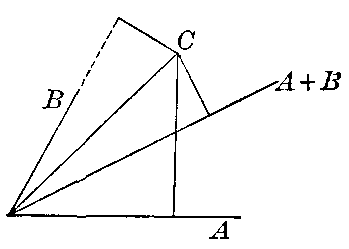
\includegraphics[width=40mm]{fig15.png}
\end{center}

Let
\begin{align*}
A &= a_1j + a_2j + a_3k, \\
B &= b_1i + b_2j + b_3k, \\
C &= c_1i + c_2j + c_3k.
\end{align*}

Since $A$ and $B$ are independent of order,\index{Distributive rule}
\begin{gather*}
A + B = (a_1 + b_1)i + (a_2 + b_2)j + (a_3 + b_3)k, \\
\intertext{consequently by the principle already established}
\begin{split}
\mathrm{S}(A + B)C &= (a_1 + b_1)c_1 + (a_2 + b_2)c_2
                                                  + (a_3 + b_3)c_3 \\
                   &= a_1c_1 + a_2c_2 + a_3c_3
                                        + b_1c_1 + b_2c_2 + b_3c_3 \\
                   &= \mathrm{S}AC + \mathrm{S}BC.
\end{split}
\end{gather*}

Similarly
\begin{align*}
\mathrm{V}(A + B)C &= \{(a_2 + b_2)c_3 - (a_3 + b_3)c_2\}i+
                                                       \text{etc.} \\
                   &= (a_2c_3 - a_3c_2)i + (b_2c_3 - b_3c_2)i
                                                          + \cdots \\
                   &= \mathrm{V}AC + \mathrm{V}BC.
\end{align*}

Hence $(A + B)C = AC + BC$.

In the same way it may be shown that if the second factor consists
of two components, $C$ and $D$, which are non-successive in their
nature, then
\begin{equation*}
(A+B)(C+D) = AC + AD + BC + BD.
\end{equation*}

When $A + B$ is a sum of component vectors
\begin{align*}
(A+B)^2 & = A^2 + B^2 + AB + BA \\
        & = A^2 + B^2 + 2\mathrm{S}AB.
\end{align*}

\small \begin{enumerate}
\item[Prob.~28.] The relative velocity of a conductor is S.W., and the
magnetic flux is N.W.; what is the direction of the electromotive
force in the conductor?

\item[Prob.~29.] The direction of the current is vertically downward,
that of the magnetic flux is West; find the direction of the
mechanical force on the conductor.

\item[Prob.~30.] A body to which a force of $2i + 3j + 4k$~pounds is
applied moves with a velocity of $5i + 6j + 7k$~feet per second;
find the rate at which work is done.

\item[Prob.~31.] A conductor $8i + 9j + 10k$~inches long is subject to
an electromotive force of $11 i +12j + 13k$~volts per inch; find the
difference of potential at the ends. \hfill (Ans.\ 326~volts.)

\item[Prob.~32.] Find the rectangular projections of the area of the
parallelogram defined by the vectors $A = 12i - 23j - 34k$ and $B =
-45i - 56j + 67k$.

\item[Prob.~33.] Show that the moment of the velocity of a body with
respect to a point is equal to the sum of the moments of its
component velocities with respect to the same point.

\item[Prob.~34.] The arm is $9i + 11j + 13k$~feet, and the force
applied at either end is $17i + 19j + 23k$~pounds weight; find the
torque.

\item[Prob.~35.] A body of 1000~pounds mass has linear velocities of
50~feet per second $\overline{30^\circ/}\!\underline{/45^\circ}$ and
60~feet per second $\overline{60^\circ/}\!\underline{/22^\circ.5}$;
find its kinetic energy.

\item[Prob.~36.] Show that if a system of area-vectors can be
represented by the faces of a polyhedron, their resultant vanishes.

\item[Prob.~37.] Show that work done by the resultant velocity is equal
to the sum of the works done by its components.
\end{enumerate} \normalsize

\chapter{Product of Three Vectors.}

Complete Product.\index{Complete product!of three vectors}---Let us
take $A = a_1i + a_2j + a_3k$, $B = b_1i + b_2j + b_3k$, and $C =
c_1i + c_2j + c_3k$. By the product of $A$, $B$, and $C$ is meant
the product of the product of $A$ and $B$ with $C$, according to the
rules p.~444).%
\index{Determinant!for second partial product of three vectors}
Hence
\begin{align*}
ABC &= (a_1b_1 + a_2b_2 + a_3b_3)(c_1i + c_2j + c_3k) \notag \\
&\quad+\Bigl\{(a_2b_3 - a_3b_2)i + (a_3b_1-a_1b_3)j +
(a_1b_2-a_2b_1)k\Bigr\}
       (c_1i+c_2j+c_3k) \notag \\
    &= (a_1b_1+a_2b_2+a_3b_3)(c_1i+c_2j+c_3k) \tag{1} \\
    &\quad+ \begin{vmatrix}
              \begin{vmatrix}
                 a_2 & a_3 \\
                 b_2 & b_3
              \end{vmatrix} &
              \begin{vmatrix}
                 a_3 & a_1 \\
                 b_3 & b_1
              \end{vmatrix} &
              \begin{vmatrix}
                 a_1 & a_2 \\
                 b_1 & b_2
              \end{vmatrix} \\
              c_1 & c_2 & c_3 \\
              i   & j   & k
            \end{vmatrix} \tag{2} \\
    &\quad+ \begin{vmatrix}
               a_1 & a_2 & a_3 \\
               b_1 & b_2 & b_3 \\
               c_1 & c_2 & c_3
             \end{vmatrix} \tag{3}
\end{align*}

\medskip Example.---Let $A = 1i + 2j + 3k$, $B = 4i + 5j + 6k$, and
$C = 7i + 8j + 9k$. Then
\begin{align*}
(1) &= (4 + 10 + 18)(7i + 8j + 9k) = 32(7i + 8j + 9k).\\
(2) &= \begin{vmatrix}
          -3 & 6 & -3 \\
           7 & 8 &  9 \\
           i & j & k
       \end{vmatrix} = 78i + 6j - 66k.\\
(3) &= \begin{vmatrix}
           1 & 2 & 3 \\
           4 & 5 & 6 \\
           7 & 8 & 9
       \end{vmatrix} = 0.
\end{align*}

\smallskip If we write $A = a\alpha$, $B = b\beta$, $C = c\gamma$,
then
\begin{align}
ABC &= abc \cos \alpha\beta \cdot \gamma \tag{1} \\
    &\quad+ abc \sin \alpha\beta \sin \overline{\alpha\beta\gamma}
           \cdot \overline{\overline{\alpha\beta}\gamma} \tag{2} \\
    &\quad+ abc \sin\alpha\beta \cos\overline{\alpha\beta}\gamma,
                                                              \tag{3}
\end{align}
where $\cos\overline{\alpha\beta}\gamma$ denotes the cosine of the
angle between the directions $\overline{\alpha\beta}$ and $\gamma$,
and $\overline{\overline{\alpha\beta}\gamma}$ denotes the direction
which is normal to both $\overline{\alpha\beta}$ and $\gamma$.

We may also write
\begin{align*}
ABC &= \mathrm{S}AB \cdot C + \mathrm{V}(\mathrm{V}AB)C
        + \mathrm{S}(\mathrm{V}AB)C \\
  &\quad \qquad (1) \qquad \qquad (2) \qquad \qquad (3)
\end{align*}

\medskip First Partial Product.---It is merely the third vector
multiplied by the scalar product of the other two, or weighted by
that product as an ordinary algebraic quantity. If the directions
are kept constant, each of the three partial products is
proportional to each of the three magnitudes.%
\index{Partial products!of three vectors}

\medskip Second Partial Product.---The second partial product may be
expressed as the difference of two products similar to the
first.%
\index{Partial products!resolution of second partial product}%
\index{Resolution!of second partial product of three vectors} For
\begin{align*}
\mathrm{V}(\mathrm{V}AB)C
  &= \{-(b_2c_2 + b_3c_3)a_1 + (c_2a_2 + c_3a_3)b_1\}i \\
  &\quad+ \{-(b_3c_3 + b_1c_1)a_2 + (c_3a_3 + c_1a_1)b_2\}j \\
  &\quad+ \{-(b_1c_1 + b_2c_2)a_3 + (c_1a_1 + c_2a_2)b_3\}k.
\end{align*}

By adding to the first of these components the null term $(b_1c_1a_1
- c_1a_1b_1)i$ we get $-\mathrm{S}BC \cdot a_1i + \mathrm{S}CA \cdot
b_1i$, and by treating the other two components similarly and adding
the results we obtain
\begin{equation*}
\mathrm{V}(\mathrm{V}AB)C = -\mathrm{S}BC \cdot A
 + \mathrm{S}CA \cdot B.
\end{equation*}

The principle here proved is of great use in solving equations (see
p.~455).

\medskip Example.---Take the same three vectors as in the preceding
example. Then
\begin{align*}
\mathrm{V}(\mathrm{V}AB)C & = -(28 + 40 + 54)(1i + 2j + 3k)\\
  &\quad +(7 + 16 + 27)(4i + 5j + 6k) \\
  & = 78i + 6j - 66k.
\end{align*}

\newpage
The determinant%
\index{Determinant!for second partial product of three vectors}
expression for this partial product may also be written in the form
\begin{equation*}
\begin{vmatrix} a_1 & a_2 \\ b_1 & b_2 \end{vmatrix}
\begin{vmatrix} c_1 & c_2 \\ i & j \end{vmatrix} +
\begin{vmatrix} a_2 & a_3 \\ b_2 & b_3 \end{vmatrix}
\begin{vmatrix} c_2 & c_3 \\ j & k \end{vmatrix} +
\begin{vmatrix} a_3 & a_1 \\ b_3 & b_1 \end{vmatrix}
\begin{vmatrix} c_3 & c_1 \\ k & i \end{vmatrix}
\end{equation*}
It follows that the frequently occurring determinant expression
\begin{equation*}
\begin{vmatrix} a_1 & a_2 \\ b_1 & b_2 \end{vmatrix}
\begin{vmatrix} c_1 & c_2 \\ d_1 & d_2 \end{vmatrix} +
\begin{vmatrix} a_2 & a_3 \\ b_2 & b_3 \end{vmatrix}
\begin{vmatrix} c_2 & c_3 \\ d_2 & d_3 \end{vmatrix} +
\begin{vmatrix} a_3 & a_1 \\ b_3 & b_1 \end{vmatrix}
\begin{vmatrix} c_3 & c_1 \\ d_3 & d_1 \end{vmatrix}
\end{equation*}
means $\mathrm{S}(\mathrm{V}AB)(\mathrm{V}CD)$.

\medskip Third Partial Product.---From the determinant expression for
the third product, we know that
\begin{align*}
\mathrm{S}(\mathrm{V}AB)C &= \mathrm{S}(\mathrm{V}BC)A =
  \mathrm{S}(\mathrm{V}CA)B \\
&= -\mathrm{S}(\mathrm{V}BA)C = -\mathrm{S}(\mathrm{V}CB)A
  = -\mathrm{S}(\mathrm{V}AC)B.
\end{align*}
Hence any of the three former may be expressed by $\mathrm{S}ABC$,
and any of the three latter by $-\mathrm{S}ABC$.

\begin{center}
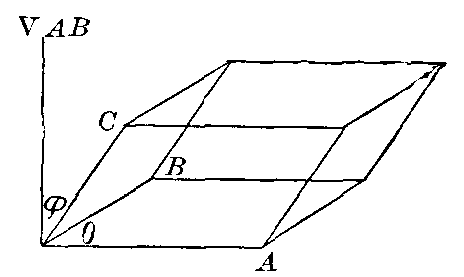
\includegraphics[width=40mm]{fig16.png}
\end{center}

The third product $\mathrm{S}(\mathrm{V}AB)C$ is represented by the
volume of the parallelepiped formed by the vectors $A, B, C$
taken in that order.%
\index{Determinant!for scalar product of three vectors} The line
$\mathrm{V}AB$ represents in magnitude and direction the area formed
by $A$ and $B$, and the product of $\mathrm{V}AB$ with the
projection of $C$ upon it is the measure of the volume in magnitude
and sign. Hence the volume formed by the three vectors has no
direction in space, but it is positive or negative according to the
cyclical order of the vectors.

In the expression $abc\, \sin \alpha\beta\, \cos \alpha\beta\gamma$
it is evident that $\sin \alpha\beta$ corresponds to $\sin \theta$,
and $\cos \alpha\beta\gamma$ to $\cos \phi$, in the usual formula
for the volume of a parallelepiped.

\medskip Example.---Let the velocity of a straight wire parallel to
itself be $V = 1000\, \underline{/30^\circ}$ centimeters per second,
let the intensity of the magnetic flux be $B = 6000\,
\underline{/90^\circ}$ lines per square centimeter, and let the
straight wire $L = 15$ centimeters $\overline{60^\circ/}\!
\underline{/45^\circ}$. Then $\mathrm{V}VB = 6000000 \sin 60^\circ\,
\overline{90^\circ/}\!\underline{/90^\circ}$ lines per centimeter
per second. Hence $\mathrm{S}(\mathrm{V}VB)L = 15 \times 6000000
\sin 60^\circ \cos \phi$ lines per second where $\cos \phi = \sin
45^\circ\, \sin 60^\circ$.

\medskip Sum of the Partial Vector Products.%
\index{Total vector product of three vectors}%
\index{Vector product!of three vectors}---By adding the first and
second partial products we obtain the total vector product of $ABC$,
which is denoted by $\mathrm{V}(ABC)$. By decomposing the second
product we obtain
\begin{equation*}
\mathrm{V}(ABC) = \mathrm{S}AB \cdot C - \mathrm{S}BC \cdot A +
\mathrm{S}CA \cdot B.
\end{equation*}
By removing the common multiplier $abc$, we get
\begin{align*}
\mathrm{V}(\alpha\beta\gamma) &= \cos \alpha\beta \cdot \gamma -
\cos \beta\gamma \cdot \alpha + \cos \gamma\alpha \cdot \beta. \\
\intertext{Similarly}
\mathrm{V}(\beta\gamma\alpha) &= \cos \beta\gamma \cdot \alpha -
\cos \gamma \alpha \cdot \beta + \cos \alpha \beta \cdot\gamma \\
\intertext{and}
\mathrm{V}(\gamma\alpha\beta) &= \cos \gamma\alpha \cdot \beta -
\cos \alpha\beta \cdot \gamma + \cos \beta\gamma \cdot \alpha.
\end{align*}

These three vectors have the same magnitude, for the square of each
is
\begin{equation*}
\cos^2\alpha\beta + \cos^2\beta\gamma + \cos^2\gamma\alpha -
2\cos\alpha\beta \cos\beta\gamma\cos\gamma\alpha,
\end{equation*}
that is, $1-\{\mathrm{S}(\alpha\beta\gamma)\}^2.$

\begin{center}
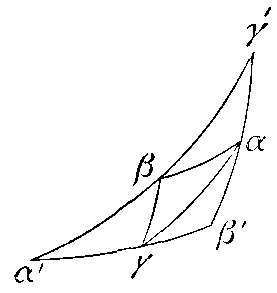
\includegraphics[width=30mm]{fig17.png}
\end{center}

They have the directions respectively of $\alpha'$, $\beta'$,
$\gamma'$, which are the corners of the triangle whose sides are
bisected by the corners $\alpha$, $\beta$, $\gamma$ of the given
triangle.

\small \begin{enumerate}
\item[Prob.~38.] Find the second partial product of $9\,
\overline{20^\circ/}\!\underline{/30^\circ}$, $10\,
\overline{30^\circ/}\!\underline{/40^\circ}$, $11\,
\overline{45^\circ/}\!\underline{/45^\circ}$. Also the third partial
product.

\item[Prob.~39.] Find the cosine of the angle between the plane of
$l_1 i + m_1 j + n_1 k$ and $l_2 i + m_2 j + n_2 k$ and the plane of
$l_3 i + m_3 j + n_3 k$ and $l_4 i + m_4 j + n_4 k$.

\item[Prob.~40.] Find the volume of the parallelepiped determined by
the vectors $100i + 50j + 25k$, $50i + 10j + 80k$, and $-75i + 40j -
80k$.

\item[Prob.~41.] Find the volume of the tetrahedron determined by the
extremities of the following vectors: $3i - 2j + 1k$, $-4i + 5j -
7k$, $3i - 7j - 2k$, $8i + 4j - 3k$.

\item[Prob.~42.] Find the voltage at the terminals of a conductor when
its velocity is 1500 centimeters per second, the intensity of the
magnetic flux is 7000 lines per square centimeter, and the length of
the conductor is 20 centimeters, the angle between the first and
second being $30^\circ$, and that between the plane of the first two
and the direction of the third $60^\circ$. \hfill (Ans.
$.91$~volts.)

\item[Prob.~43.] Let $\alpha = \overline{20^\circ/}\!
\underline{/10^\circ}$, $\beta = \overline{30^\circ/}\!
\underline{/25^\circ}$, $\gamma=\overline{40^\circ/}\!
\underline{/35^\circ}$. Find $\mathrm{V}\alpha\beta\gamma$, and
deduce $\mathrm{V}\beta\gamma\alpha$ and
$\mathrm{V}\gamma\alpha\beta$.
\end{enumerate} \normalsize

\chapter{Composition of Quantities.}

A number of homogeneous quantities are simultaneously located at
different points; it is required to find how to add or compound
them.

\begin{center}
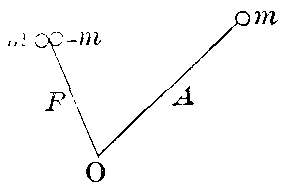
\includegraphics[width=40mm]{fig18.png}
\end{center}

\smallskip Addition of a Located Scalar Quantity.---Let $m_A$ denote a
mass $m$ situated at the extremity of the radius-vector $A$. A mass
$m-m$ may be introduced at the extremity of any radius-vector R, so
that
\begin{align*}
m_A &= (m - m)_R + m_A \\
    &= m_R + m_A - m_R \\
    &= m_R + m(A - R).
\end{align*}
Here $A-R$ is a simultaneous sum, and denotes the radius-vector from
the extremity of $R$ to the extremity of $A$. The product $m(A - R)$
is what Clerk Maxwell called a mass-vector, and means the directed
moment of $m$ with respect to the extremity of $R$.\index{Maxwell}
The equation states that the mass $m$ at the extremity of the vector
$A$ is equivalent to the equal mass at the extremity of $R$,
together with the said mass-vector applied at the extremity of $R$.
The equation expresses a physical of mechanical
principle.\index{Composition!of
mass-vectors}\index{Mass-vector}\index{Mass-vector!composition of}

Hence for any number of masses, $m_1$ at the extremity of $A_1$,
$m_2$ at the extremity of $A_2$, etc.,
\begin{equation*}
\sum m_A = \sum m_R + \sum\Bigl\{m(A - R)\Bigr\},
\end{equation*}
where the latter term denotes the sum of the mass-vectors treated as
simultaneous vectors applied at a common point. Since
\begin{align*}
\sum \bigl\{m(A-R)\bigr\} &= \sum m A - \sum mR \\
                &= \sum m A - R\sum m,
\end{align*}
the resultant moment will vanish\index{Couple of forces!condition
for couple vanishing} if
\begin{equation*}
R = \frac{\sum mA}{\sum m},\quad\text{or}\quad R \sum m = \sum mA
\end{equation*}

\smallskip Corollary.\index{Couple of forces}---Let
\begin{align*}
R &= xi + yj + zk, \\
\intertext{and}
A &= a_1j + b_1j+c_1k; \\
\intertext{then the above condition may be written as}
xi + yj + zk &= \frac{\sum\bigl\{m(ai + bj + ck)\bigr\}}{\sum m} \\
             &= \frac{\sum (ma)\cdot i}{\sum m} +
                \frac{\sum (mb)\cdot j}{\sum m} +
                \frac{\sum (mc)\cdot k}{\sum m}; \\
\intertext{therefore}
           x &= \frac{\sum (ma)}{\sum m},\
           y  = \frac{\sum (mb)}{\sum m},\
           z  = \frac{\sum (mc)}{\sum m}. \\
\end{align*}

Example.---Given $5$ pounds at $10$ feet $\overline{45^\circ/}\!
\underline{/30^\circ}$ and $8$ pounds at $7$ feet
$\overline{60^\circ/}\!\underline{/45^\circ}$; find the moment when
both masses are transferred to $12$ feet $\overline{75^\circ/}\!
\underline{/60^\circ}$.
\begin{align*}
m_1A_1 &= 50(\cos 30^\circ i + \sin 30^\circ \cos 45^\circ j
          + \sin 30^\circ \sin 45^\circ k), \\
m_1A_1 &= 56(\cos 45^\circ i + \sin 45^\circ \cos 60^\circ j
          + \sin 45^\circ \sin 60^\circ k), \\
(m_1 + m_2)R &= 156(\cos 60^\circ i + \sin 60^\circ \cos 75^\circ j
          + \sin 60^\circ \sin 75^\circ k),\\
\text{moment} &=  m_1 A_1 + m_2A_2 -(m_1 + m_2)R.
\end{align*}

\newpage
\begin{center}
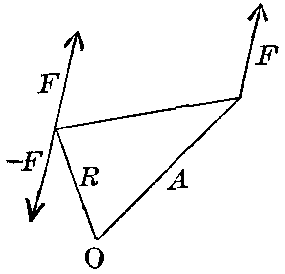
\includegraphics[width=40mm]{fig19.png}
\end{center}

\smallskip Composition of a Located Vector
Quantity.\index{Composition!of located vectors}\index{Located
vectors}---Let $F_A$ denote a force applied at the extremity of the
radius-vector $A$. As a force $F-F$ may introduced at the extremity
of any radius-vector $R$, we have
\begin{align*}
F_A &= (F - F) + F_A \\
    &= F_R + \mathrm{V}(A-R)F.
\end{align*}

This equation asserts that a force $F$ applied at the extremity of
$A$ is equivalent to an equal force applied at the extremity of $R$
together with a couple whose magnitude and direction are given by
the vector product of the radius-vector from the extremity of $R$ to
the extremity of $A$ and the force.

Hence for a system of forces applied at different points, such as
$F_1$ at $A_1$, $F_2$ at $A_2$, etc., we obtain
\begin{align*}
\sum \left(F_A\right) &= \sum \left(F_R\right)
                         + \sum \mathrm{V}\left(A - R\right)F  \\
           &= \left(\sum F\right)_R
                         + \sum \mathrm{V}\left(A - R\right)F. \\
\intertext{Since}
\sum \mathrm{V}\left(A - R\right)F
                        &= \sum \mathrm{V}AF - \sum \mathrm{V}RF \\
                        &= \sum \mathrm{V}AF - \mathrm{V}R \sum F \\
\intertext{the condition for no resultant couple is} \mathrm{V} R
\sum F &= \sum \mathrm{V} A F,
\end{align*}
which requires $\sum F$ to be normal to $\sum \mathrm{V} A F$.

\medskip Example.---Given a force $1i + 2j + 3k$ pounds weight at $4i
+ 5j + 6k$ feet, and a force of $7i + 9j + 11k$ pounds weight at
$10i + 12j + 14k$ feet; find the torque which must be supplied when
both are transferred to $2i + 5j + 3k$, so that the effect may be
the same as before.\index{Torque}
\begin{align*}
\mathrm{V} A_1 F_1  &= 3i - 6j + 3k, \\
\mathrm{V} A_2 F_2  &= 6i - 12j + 6k, \\
\sum \mathrm{V} A F &= 9i - 18j + 9k, \\
\sum F              &= 8i + 11j + 14k, \\
\mathrm{V} R \sum F &= 37i - 4j - 18k, \\
\text{Torque}       &= -28i - 14j + 27k.
\end{align*}

By taking the vector product of the above equal vectors with the
reciprocal of $\sum F$ we obtain
\begin{equation*}
\mathrm{V}\left\{ \left(\mathrm{V} R \sum F\right)
                \frac{1}{\sum F} \right\}
= \mathrm{V}\left\{ \left(\sum \mathrm{V} A F \right)
                \frac{1}{\sum F} \right\}.
\end{equation*}

By the principle previously established the left member resolves
into $-R + \mathrm{S}R\dfrac{1}{\sum F} \cdot \sum F$; and the right
member is equivalent to the complete product on account of the two
factors being normal to one another; hence
\begin{align}
-R &+ \mathrm{S} R \frac{1}{\sum F} \cdot \sum F
   = \sum \left(\mathrm{V} A F \right) \frac{1}{\sum F}; \notag \\
\intertext{that is,}
R &= \frac{1}{\sum F}\sum \left(\mathrm{V}AF \right) \tag{1} \\
  &\quad+ \mathrm{S}R\frac{1}{\sum F} \cdot \sum F \tag{2}.
\end{align}

\begin{center}
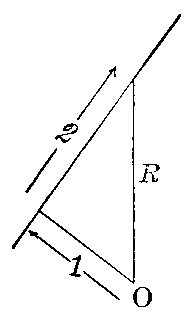
\includegraphics[width=25mm]{fig20.png}
\end{center}

The extremity of $R$ lies on a straight line whose perpendicular is
the vector (1) and whose direction is that of the resultant force.
The term (2) means the projection of $R$ upon that line.

The condition for the central axis\index{Central axis} is that the
resultant force and the resultant couple should have the same
direction; hence it is given by
\begin{align*}
\mathrm{V}\left\{\sum \mathrm{V}AF - \mathrm{V}R\sum F\right\}
  \sum F = 0; \\
\intertext{that is}
\mathrm{V}\left(\mathrm{V}R\sum F \right)\sum F =
  \mathrm{V}\left(\sum AF \right)\sum F.
\end{align*}

By expanding the left member according to the same principle as
above, we obtain
\begin{equation*}
-\left(\sum F\right)^2R + \mathrm{S}R\sum F \cdot \sum F
  = V\left(\sum AF \right)\sum F;
\end{equation*}
therefore
\begin{align*}
R &= \frac{1}{\left(\sum F \right)^2}\mathrm{V}\sum F
     \left(\mathrm{V}\sum AF\right) +
     \frac{\mathrm{S}R\sum F}{\left(\sum F\right)^2} \cdot \sum F \\
  &= \mathrm{V}\left(\frac{1}{\sum F}\right)(\mathrm{V}\sum AF) +
       \mathrm{S}R\frac{1}{\sum F} \cdot \sum F.
\end{align*}

This is the same straight line as before, only no relation is now
imposed on the directions of $\sum F$ and $\sum \mathrm{V}AF$; hence
there always is a central axis.

\medskip Example.---Find the central axis for the system of forces in
the previous example. Since $\sum F = 8i + 11j + 14k$, the direction
of the line is
\begin{equation*}
\frac{8i + 11j + 14k}{\sqrt{64 + 121 + 196}}.
\end{equation*}

Since $\dfrac{1}{\sum F} = \dfrac{8i + 11j + 14k}{381}$ and $\sum
\mathrm{V}AF = 9i - 18j + 9k$, the perpendicular to the line is
\begin{equation*}
\mathrm{V}\,\frac{8i + 11j + 14k}{381}\, 9i - 18j + 9k =
  \frac{1}{381}\,\{351i + 54j -243k\}.
\end{equation*}

\small \begin{enumerate}
\item[Prob.~44.] Find the moment at $\overline{90^\circ/}\!
\underline{/270^\circ}$ of 10~pounds at 4~feet
$\overline{10^\circ/}\!\underline{/20^\circ}$ and 20~pounds at
5~feet $\overline{30^\circ/}\!\underline{/120^\circ}$.

\item[Prob.~45.] Find the torque for $4i + 3j + 2k$ pounds weight at
$2i - 3j + 1k$ feet, and $2i - 1k - 1k$ pounds weight at $-3i + 4j +
5k$~feet when transferred to $-3i -2j -4k$ feet.

\item[Prob.~46.] Find the central axis in the above case.

\item[Prob.~47.] Prove that the mass-vector drawn from any origin to a
mass equal to that of the whole system placed at the center of mass
of the system is equal to the sum of the mass-vectors drawn from the
same origin to all the particles of the system.
\end{enumerate} \normalsize

\chapter{Spherical Trigonometry.}\index{Spherical trigonometry}

\begin{center}
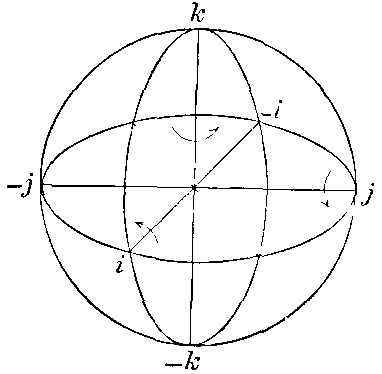
\includegraphics[width=40mm]{fig21.png}
\end{center}

Let $i$, $j$, $k$ denote three mutually perpendicular axes. In order
to distinguish clearly between an axis and a quadrantal version
round it, let $i^\frac{\pi}{2}$, $j^\frac{\pi}{2}$,
$k^\frac{\pi}{2}$ denote quadrantal versions in the positive sense
about the axes $i$, $j$, $k$ respectively.\index{Meaning!of
$\frac{1}{2}\pi$ as index} The directions of positive version are
indicated by the arrows.

By $i^\frac{\pi}{2}i^\frac{\pi}{2}$ is meant the product of two
quadrantal versions round $i$; it is equivalent to a semicircular
version round $i$; hence $i^\frac{\pi}{2}i^\frac{\pi}{2} = i^\pi =
-$. Similarly $j^\frac{\pi}{2}j^\frac{\pi}{2}$ means the product of
two quadrantal versions round $j$, and
$j^\frac{\pi}{2}j^\frac{\pi}{2}=j^\pi=-$. Similarly
$k^\frac{\pi}{2}k^\frac{\pi}{2}=k^\pi=-$.

By $i^\frac{\pi}{2}j^\frac{\pi}{2}$ is meant a quadrant round $i$
followed by a quadrant round $j$; it is equivalent to the quadrant
from $j$ to $i$, that is, to $-k^\frac{\pi}{2}$. But
$j^\frac{\pi}{2}i^\frac{\pi}{2}$ is equivalent to the quadrant from
$-i$ to $-j$, that is, to $k^\frac{\pi}{2}$. Similarly for the other
two pairs of products. Hence we obtain the following

\begin{center}
Rules for Versors.\index{Rules!for versors}\index{Versor!rules for}
\end{center}
\begin{gather*}
i^\frac{\pi}{2}i^\frac{\pi}{2} = -, \quad
j^\frac{\pi}{2}j^\frac{\pi}{2} = -, \quad
k^\frac{\pi}{2}k^\frac{\pi}{2} = -, \\
i^\frac{\pi}{2}j^\frac{\pi}{2} = -k^\frac{\pi}{2}, \quad
j^\frac{\pi}{2}i^\frac{\pi}{2} =  k^\frac{\pi}{2}, \\
j^\frac{\pi}{2}k^\frac{\pi}{2} = -i^\frac{\pi}{2}, \quad
k^\frac{\pi}{2}j^\frac{\pi}{2} =  i^\frac{\pi}{2}  \\
k^\frac{\pi}{2}i^\frac{\pi}{2} = -j^\frac{\pi}{2}, \quad
i^\frac{\pi}{2}k^\frac{\pi}{2} =  j^\frac{\pi}{2}.
\end{gather*}

The meaning of these rules will be seen from the following
application. Let $li + mj + nk$ denote any axis, then $(li + mj +
nk)^\frac{\pi}{2}$ denotes a quadrant of angle round that axis. This
quadrantal version can be decomposed into the three rectangular
components $li^\frac{\pi}{2}$, $mj^\frac{\pi}{2}$,
$nk^\frac{\pi}{2}$; and these components are not successive
versions, but the parts of one version.\index{Versor!components of}
Similarly any other quadrantal version $(l'i + m'j +
n'j)^\frac{\pi}{2}$ can be resolved into
$l'i^\frac{\pi}{2}$, $m'j^\frac{\pi}{2}$, $n'k^\frac{\pi}{2}$.%
\index{Product!of two quadrantal versors}%
\index{Rules!for expansion of product of two quadrantal versors} By
applying the above rules, we obtain
\begin{align*}
(li &+ mj + nk)^\frac{\pi}{2}(l'i + m'j + n'k)^\frac{\pi}{2} \\
    &= (li^\frac{\pi}{2} + mj^\frac{\pi}{2} + nk^\frac{\pi}{2})
         (l'i^\frac{\pi}{2} + m'j^\frac{\pi}{2} + n'k^\frac{\pi}{2}) \\
    &= -(ll' + mm' + nn') -(mn' - m'n)i^\frac{\pi}{2}
            - (nl' - n'l)j^\frac{\pi}{2} -(lm' - l'm)k^\frac{\pi}{2} \\
    &= -(ll' + mm' + nn')-\bigl\{(mn' - m'n)i + (nl' - n'l)j
             +(lm' - l'm)k\bigr\}^\frac{\pi}{2}.
\end{align*}

\begin{center}
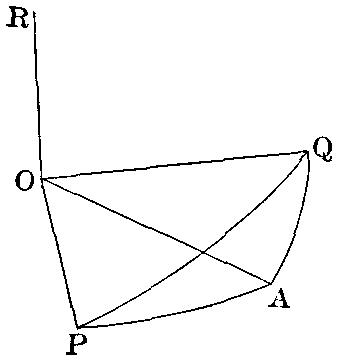
\includegraphics[width=40mm]{fig22.png}
\end{center}

\smallskip Product of Two Spherical Versors.%
\index{Product!of two spherical versors}%
\index{Spherical versor}%
\index{Spherical versor!product of two}%
\index{Versor!product of two quadrantal}%
\index{Versor!product of two general spherical}---Let $\beta$ denote
the axis and $b$ the ratio of the spherical versor $PA$, then the
versor itself is expressed by $\beta^b$. Similarly let $\gamma$
denote the axis and $c$ the ratio of the spherical versor $AQ$, then
the versor itself is expressed by $\gamma^c$.

Now
\begin{align*}
\beta^b &= \cos b + \sin b \cdot \beta^\frac{\pi}{2}, \\
\intertext{and}
\gamma^c &= \cos c + \sin c \cdot \gamma^\frac{\pi}{2}; \\
\intertext{therefore}
\beta^b\gamma^c &= (\cos b + \sin b \cdot
\beta^\frac{\pi}{2})(\cos c + \sin c \cdot \gamma^\frac{\pi}{2}) \\
 &= \cos b \cos c + \cos b \sin c \cdot \gamma^\frac{\pi}{2}
     + \cos c \sin b \cdot \beta^\frac{\pi}{2}
     + \sin b \sin c \cdot \beta^\frac{\pi}{2}\gamma^\frac{\pi}{2}.
\end{align*}

\smallskip But from the preceding paragraph
\begin{align}
\beta^\frac{\pi}{2}\gamma^\frac{\pi}{2} &= -\cos\beta\gamma -
  \sin\beta\gamma \cdot
                      \overline{\beta\gamma}^\frac{\pi}{2}; \notag \\
\intertext{therefore}
\beta^b\gamma^c &=
            \cos b \cos c - \sin b \sin c \cos \beta\gamma \tag{1} \\
&\quad+ \{\cos b \sin c \cdot \gamma + \cos c \sin b \cdot \beta -
\sin b \sin c \sin \beta\gamma \cdot
\overline{\beta\gamma}\}^\frac{\pi}{2}. \tag{2}
\end{align}

\smallskip The first term gives the cosine of the product versor; it
is equivalent to the fundamental theorem of spherical
trigonometry,\index{Spherical trigonometry!fundamental theorem of}
namely,
\begin{equation*}
\cos a = \cos b \cos c + \sin b \sin c \cos A,
\end{equation*}
where $A$ denotes the external angle instead of the angle included
by the sides.

The second term is the directed sine of the angle; for the square of
(2) is equal to 1 minus the square of (1), and its direction is
normal to the plane of the product angle.\footnote{Principles of
Elliptic and Hyperbolic Analysis, p.~2.}

\medskip Example.---Let $\beta = \overline{30^\circ/}\!
\underline{/45^\circ}$ and $\gamma = \overline{60^\circ/}\!
\underline{/30^\circ}$. Then
\begin{align*}
\cos \beta\gamma &= \cos 45^\circ \cos 30^\circ + \sin 45^\circ \sin
30^\circ \cos 30^\circ, \\
\intertext{and}
\sin \beta\gamma &\cdot \overline{\beta\gamma} =
  \mathrm{V}\beta\gamma; \\
\intertext{but}
\beta &= \cos 45^\circ i + \sin 45^\circ \cos
30^\circ j + \sin 45^\circ \sin 30^\circ k, \\
\intertext{and}
\gamma &= \cos 30^\circ i + \sin 30^\circ \cos
60^\circ j + \sin 30^\circ \sin 60^\circ k; \\
\intertext{therefore}
\mathrm{V}\beta\gamma & = \{\sin 45^\circ \cos 30^\circ
   \sin 30^\circ \sin 60^\circ -\sin 45^\circ \sin 30^\circ
   \sin 30^\circ \cos 60^\circ \}i \\
&\quad+ \{ \sin 45^\circ \sin 30^\circ \cos 30^\circ -
   \cos 45^\circ \sin 30^\circ \sin 60^\circ \} j \\
&\quad+ \{ \cos 45^\circ \sin 30^\circ \cos 60^\circ -
   \sin 45^\circ \cos 30^\circ \cos 30^\circ \} k.
\end{align*}

\medskip Quotient of Two Spherical Versors.%
\index{Spherical versor!quotient of two}---The reciprocal of a given
versor is derived by changing the sign of the index; $\gamma^{-c}$
is the reciprocal of $\gamma^c$. As $\beta^b = \cos b + \sin b \cdot
\beta^\frac{\pi}{2}$, and $y^{-c} = \cos c - \sin c \cdot
\gamma^\frac{\pi}{2}$,
\begin{align*}
\beta^b\gamma^{-c} &= \cos b \cos c +
                                    \sin b \sin c \cos \beta\gamma \\
  &+\{\cos c \sin b \cdot \beta - \cos b \sin c \cdot \gamma
      + \sin b \sin c \sin \beta\gamma \cdot
      \overline{\beta\gamma}\}^\frac{\pi}{2}.
\end{align*}

\begin{center}
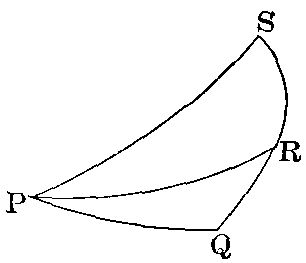
\includegraphics[width=30mm]{fig23.png}
\end{center}

\smallskip Product of Three Spherical Versors.%
\index{Product!of three spherical versors}%
\index{Spherical versor!product of three}%
\index{Versor!product of three general spherical}---Let $\alpha^a$
denote the versor $PQ$, $\beta^b$ the versor $QR$, and $\gamma^c$
the versor $RS$; then $\alpha^a\beta^b\gamma^c$ denotes $PS$. Now
$\alpha^a\beta^b\gamma^c$
\begin{align}
=&(\cos a + \sin a \cdot\alpha^\frac{\pi}{2})
  (\cos b + \sin b \cdot\beta^\frac{\pi}{2})
  (\cos c + \sin c \cdot\gamma^\frac{\pi}{2}) \notag \\
=& \cos a\cos b\cos c \tag{1} \\
 & + \cos a \cos b \sin c \cdot \gamma^\frac{\pi}{2} +
     \cos a \cos c \sin b \cdot \beta^\frac{\pi}{2} +
     \cos b \cos c \sin a \cdot \alpha^\frac{\pi}{2} \tag{2} \\
 & + \cos a \sin b \sin c \cdot
                            \beta^\frac{\pi}{2}\gamma^\frac{\pi}{2} +
     \cos b \sin a \sin c \cdot
                   \alpha^\frac{\pi}{2}\gamma^\frac{\pi}{2} \notag \\
 & \qquad + \cos c \sin a \sin b \cdot
                              \alpha^\frac{\pi}{2}\beta^\frac{\pi}{2}
 \tag{3} \\
 & + \sin a \sin b \sin c \cdot
          \alpha^\frac{\pi}{2}\beta^\frac{\pi}{2}\gamma^\frac{\pi}{2}
\tag{4}
\end{align}

The versors in (3) are expanded by the rule already obtained,
namely,
\begin{equation*}
\beta^\frac{\pi}{2}\gamma^\frac{\pi}{2} = -\cos \beta\gamma -\sin
\beta\gamma \cdot \overline{\beta\gamma}^\frac{\pi}{2}.
\end{equation*}

The versor of the fourth term is
\begin{align*}
\alpha^\frac{\pi}{2}\beta^\frac{\pi}{2}\gamma^\frac{\pi}{2} &=
  -(\cos\alpha\beta + \sin\alpha\beta \cdot
      \overline{\alpha\beta}^\frac{\pi}{2}) \gamma^\frac{\pi}{2} \\
&= -\cos\alpha\beta \cdot \gamma^\frac{\pi}{2} +
  \sin\alpha\beta\cos\overline{\alpha\beta}\gamma +
  \sin\alpha\beta\sin\overline{\alpha\beta}\gamma \cdot
  \overline{\overline{\alpha\beta}\gamma}^\frac{\pi}{2}.
\end{align*}

Now $\sin\alpha\beta \sin\overline{\alpha\beta}\gamma \cdot
\overline{\overline{\alpha\beta}\gamma} = \cos\alpha\gamma \cdot
\beta - \cos\beta\gamma \cdot \alpha$ (p.~451), hence the last term
of the product, when expanded, is
\begin{equation*}
\sin a\sin b\sin c\left\{-\cos \alpha\beta \cdot
  \gamma^\frac{\pi}{2}
+ \cos\alpha\gamma \cdot \beta^\frac{\pi}{2}
- \cos\beta\gamma \cdot \alpha^\frac{\pi}{2}
+ \cos\overline{\alpha\beta}\gamma\right\}.
\end{equation*}

\newpage
Hence
\begin{align*}
\cos\alpha^a\beta^b\gamma^c &=
  \cos a\cos b\cos c - \cos a\sin b\sin c\cos \beta\gamma \\
&- \cos b\sin a\sin c\cos \alpha\gamma -
                                \cos c\sin a\sin b\cos \alpha\beta \\
&+ \sin a\sin b\sin c\sin \alpha\beta\cos\alpha\beta\gamma, \\
\intertext{and, letting Sin denote the directed sine,}
\Sin \alpha^a\beta^b\gamma^c &=
  \cos a \cos b \sin c \cdot \gamma +
                                  \cos a \cos c \sin b \cdot \beta \\
&+ \cos b \cos c \sin a \cdot \alpha -
  \cos a \sin b \sin c \sin \beta\gamma \cdot
                                            \overline{\beta\gamma} \\
&- \cos b \sin a \sin c \sin \alpha\gamma \cdot
                                           \overline{\alpha\gamma} \\
&- \cos c \sin a \sin b \sin \alpha\beta \cdot
                                            \overline{\alpha\beta} \\
&- \sin a \sin b \sin c\left\{\cos\alpha\beta \cdot \gamma -
  \cos \alpha\gamma \cdot  \beta + \cos \beta\gamma \cdot
  \alpha\right\}.\footnotemark
\end{align*}
\footnotetext{In the above case the three axes of the successive
angles are not perfectly independent, for the third angle must begin
where the second leaves off. But the theorem remains true when the
axes are independent; the factors are then quaternions in the most
general sense.}

Extension of the Exponential Theorem to Spherical
Trigonometry.\index{Binomial theorem in spherical analysis}%
\index{Exponential theorem in spherical trigonometry}---It has been
shown (p.~458) that
\begin{align*}
\cos\beta^b\gamma^c &= \cos b\cos c - \sin b\sin c\cos \beta\gamma
\intertext{and}
\left(\sin \beta^b\gamma^c\right)^\frac{\pi}{2} &=
  \cos c \sin b \cdot \beta^\frac{\pi}{2} + \cos b \sin c \cdot
  \gamma^\frac{\pi}{2} - \sin b \sin c \sin \beta\gamma \cdot
  \overline{\beta\gamma}^\frac{\pi}{2}.
\end{align*}

Now
\begin{align*}
\cos b &= 1 - \frac{b^2}{2!} + \frac{b^4}{4!} - \frac{b^6}{6!} +
   \text{ etc.} \\
\intertext{and} \sin b &= b - \frac{b^3}{3!} + \frac{b^5}{5!} -
   \text{ etc.}
\end{align*}\index{Spherical trigonometry!binomial theorem}

\smallskip Substitute these series for $\cos b$, $\sin b$, $\cos c$,
and $\sin c$ in the above equations, multiply out, and group the
homogeneous terms together. It will be found that
\begin{align*}
\cos\beta^b\gamma^c = 1
  &- \frac{1}{2!}\{b^2 + 2bc\cos\beta\gamma + c^2\} \\
  &+ \frac{1}{4!}\{b^4 + 4b^3c\cos\beta\gamma + 6b^2c^2 +
       4bc^3\cos\beta\gamma + c^4\} \\
  &- \frac{1}{6!}\{b^6 + 6b^5c\cos\beta\gamma + 15b^4c^2 +
       20b^3c^3\cos\beta\gamma \\
  & \qquad \qquad + 15b^2c^4 + 6bc^5\cos\beta\gamma + c^6\} + \ldots,
\end{align*}
where the coefficients are those of the binomial theorem, the only
difference being that $\cos \beta\gamma$ occurs in all the odd terms
as a factor. Similarly, by expanding the terms of the sine, we
obtain
\begin{align*}
(\Sin \beta^b\gamma^c)^\frac{\pi}{2} &=
    b \cdot \beta^\frac{\pi}{2} + c \cdot \gamma^\frac{\pi}{2} -
    bc \sin \beta\gamma \cdot \overline{\beta\gamma}^\frac{\pi}{2} \\
&\quad- \frac{1}{3!}\{b^3 \cdot \beta^\frac{\pi}{2} + 3b^2c \cdot
      \gamma^\frac{\pi}{2} +
    3bc^2 \cdot \beta^\frac{\pi}{2} + c^3 \cdot
                                            \gamma^\frac{\pi}{2}\} \\
&\quad+ \frac{1}{3!}\{bc^3 + b^3c\}
      \sin\beta\gamma \cdot \overline{\beta\gamma}^\frac{\pi}{2} \\
&\quad+ \frac{1}{5!}\{b^5 \cdot \beta^\frac{\pi}{2} +
      5b^4c \cdot \gamma^\frac{\pi}{2} + 10b^3c^2 \cdot
      \beta^\frac{\pi}{2} \\
&\quad\qquad + 10b^2c^3\cdot\gamma^\frac{\pi}{2} + 5bc^4 \cdot
      \beta^\frac{\pi}{2}
      + c^5 \cdot \gamma^\frac{\pi}{2} \\
&\quad- \frac{1}{5!}\left\{b^5c + \frac{5\cdot 4}{2\cdot 3}b^2c^3 +
      bc^5\right\} \sin\beta\gamma \cdot
      \overline{\beta\gamma}^\frac{\pi}{2} - \ldots
\end{align*}

By adding these two expansions together we get the expansion for
$\beta^b\gamma^c$, namely,
\begin{align*}
\beta^b\gamma^c = 1 &+ b \cdot\beta^\frac{\pi}{2} +
                                        c\cdot\gamma^\frac{\pi}{2} \\
&- \frac{1}{2!}\{b^2 + 2bc(\cos\beta\gamma + \sin\beta\gamma \cdot
  \overline{\beta\gamma}^\frac{\pi}{2}) + c^2\} \\
&- \frac{1}{3!}\{b^3 \cdot \beta^\frac{\pi}{2} + 3b^2c
\cdot\gamma^\frac{\pi}{2}
  + 3bc^2 \cdot \beta^\frac{\pi}{2} + c^3 \cdot
                                            \gamma^\frac{\pi}{2}\} \\
&+ \frac{1}{4!}\{b^4 + 4b^3c(\cos\beta\gamma + \sin\beta\gamma \cdot
    \overline{\beta\gamma}^\frac{\pi}{2}) + 6b^2c^2 \\
&\qquad + 4bc^3(\cos\beta\gamma+\sin\beta\gamma \cdot
  \overline{\beta\gamma}^\frac{\pi}{2}) + c^4\} + \ldots
\end{align*}

By restoring the minus, we find that the terms on the second line
can be thrown into the form
\begin{gather*}
\frac{1}{2!} \left\{ b^2 \cdot \beta^{\pi} + 2bc \cdot
\beta^{\frac{\pi}{2}}\gamma^{\frac{\pi}{2}} + c^{2} \cdot
\gamma^{\pi} \right\}, \\
\intertext{and this is equal to}
\frac{1}{2!} \left\{ b \cdot \beta^{\frac{\pi}{2}} +
  c \cdot \gamma^{\frac{\pi}{2}} \right\}^2, \\
\intertext{where we have the square of a sum of successive terms. In
a similar manner the terms on the third line can be restored to}
b^3 \cdot \beta^\frac{3\pi}{2} +
  3b^2c \cdot \beta^\pi \gamma^\frac{\pi}{2} +
  3bc^2 \cdot \beta^\frac{\pi}{2}\gamma^\pi +
  c^3 \cdot \gamma^{3(\frac{\pi}{2})}, \\
\intertext{that is,}
\frac{1}{3!} \left\{ b \cdot \beta^\frac{\pi}{2} +
  c \cdot \gamma^\frac{\pi}{2} \right\} ^3.
\end{gather*}

Hence
\begin{align*}
\beta^b\gamma^c &= 1 + b \cdot \beta^\frac{\pi}{2}
      + c \cdot \gamma^\frac{\pi}{2}
    + \frac{1}{2!} \left\{ b \cdot \beta^\frac{\pi}{2}
      + c \cdot \gamma^\frac{\pi}{2} \right\} ^2 \\
   &\qquad + \frac{1}{3!} \left\{ b \cdot \beta^\frac{\pi}{2}
      + c \cdot \gamma^\frac{\pi}{2} \right\} ^3
      + \frac{1}{4!} \left\{ b \cdot \beta^\frac{\pi}{2}
      + c \cdot \gamma^\frac{\pi}{2} \right\} ^4 + \ldots \\
&= e ^{b \cdot \beta^\frac{\pi}{2} + c \cdot
\gamma^\frac{\pi}{2}}.\footnotemark
\end{align*}
\footnotetext{At page 386 of his Elements of Quaternions, Hamilton
says: ``In the present theory of diplanar quaternions we cannot
expect to find that the sum of the logarithms of any two proposed
factors shall be generally equal to the logarithm of the product;
but for the simpler and earlier case of coplanar quaternions, that
algebraic property may be considered to exist, with due modification
for multiplicity of value.'' He was led to this view by not
distinguishing between vectors and quadrantal quaternions and
between simultaneous and successive addition. The above
demonstration was first given in my paper on ``The Fundamental
Theorems of Analysis generalized for Space.'' It forms the key to
the higher development of space analysis.}%
\index{Exponential theorem in spherical trigonometry!Hamilton's
view}%
\index{Hamilton's!view of exponential theorem in spherical analysis}

Extension of the Binomial Theorem.---We have proved above that
$e^{b\beta^\frac{\pi}{2}} e^{c\gamma^\frac{\pi}{2}} =
e^{b\beta^\frac{\pi}{2} + c\gamma^\frac{\pi}{2}}$ provided that the
powers of the binomial are expanded as due to a successive sum, that
is, the order of the terms in the binomial must be preserved. Hence
the expansion for a power of a successive binomial is given by
\begin{multline*}
\left\{ b \cdot \beta^\frac{\pi}{2} +
        c \cdot \gamma^\frac{\pi}{2} \right\}^n =
b^n \cdot \beta^{n^\frac{\pi}{2}} + nb^{n-1}c  \cdot
    \beta^{(n-1)(\frac{\pi}{2})} \gamma^\frac{\pi}{2} \\
+ \frac{n(n-1)}{1 \cdot 2} b^{n-2} c^2 \cdot
    \beta^{(n-2)(\frac{\pi}{2})} \gamma^\pi + \text{etc.}
\end{multline*}

\smallskip Example.---Let $b = \frac{1}{10}$ and $c = \frac{1}{5}$,
$\beta = \overline{30^\circ/}\!\underline{/45^\circ}$, $\gamma =
\overline{60^\circ/}\!\underline{/30^\circ}$.
\begin{align*}
(b \cdot \beta^\frac{\pi}{2} + c \cdot \gamma^\frac{\pi}{2})^2
&= -\{b^2 + c^2 + 2bc\cos\beta\gamma
      + 2bc(\sin\beta\gamma)^\frac{\pi}{2} \} \\
&= -\left(\tfrac{1}{100} + \tfrac{1}{25}
      + \tfrac{2}{50}\cos\beta\gamma\right)
      - \tfrac{2}{50}\left(\sin\beta\gamma\right)^\frac{\pi}{2}.
\end{align*}
Substitute the calculated values of $\cos \beta\gamma$ and
$\sin \beta\gamma$ (page 459).

\small \begin{enumerate}
\item[Prob.~48.] Find the equivalent of a quadrantal version round
$\dfrac{\sqrt{3}}{2}i + \dfrac{1}{2\sqrt{2}}j +
\dfrac{1}{2\sqrt{2}}k$ followed by a quadrantal version round
$\dfrac{1}{2}i + \dfrac{\sqrt{3}}{4}j + \dfrac{3}{4}k$.

\item[Prob.~49.] In the example on p.~459 let $b=25^\circ$ and $c =
50^\circ$; calculate out the cosine and the directed sine of the
product angle.

\item[Prob.~50.] In the above example calculate the cosine and the
directed sine up to and inclusive of the fourth power of the
binomial. \hfill (Ans.~$\cos =.9735$.)

\item[Prob.~51.] Calculate the first four terms of the series when
$b = \frac{1}{50}$, $c = \frac{1}{100}$, $\beta =
\overline{0^\circ/}\! \underline{/0^\circ}$, $\gamma =
\overline{90^\circ/}\! \underline{/90^\circ}$.

\item[Prob.~52.] From the fundamental theorem of spherical
trigonometry deduce the polar theorem with respect to both the
cosine and the directed sine.

\item[Prob.~53.] Prove that if $\alpha^a, \beta^b, \gamma^c$ denote
the three versors of a spherical triangle, then
\begin{equation*}
\frac{\sin\beta\gamma}{\sin a} = \frac{\sin\gamma\alpha}{\sin b} =
  \frac{\sin\alpha\beta}{\sin c}.
\end{equation*}
\end{enumerate} \normalsize

\chapter{Composition of Rotations.}

\begin{center}
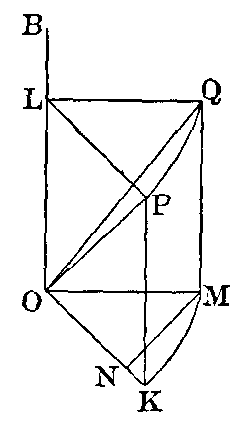
\includegraphics[width=25mm]{fig24.png}
\end{center}

A version refers to the change of direction of a line, but a
rotation refers to a rigid body. The composition of rotations is a
different matter from the composition of versions.%
\index{Composition!of finite rotations}%
\index{Rotations, finite}

\medskip Effect of a Finite Rotation on a Line.---Suppose that a
rigid body rotates $\theta$~radians round the axis $\beta$ passing
through the point $O$, and that $R$ is the radius vector from $O$ to
some particle. In the diagram $OB$ represents the axis $\beta$, and
$OP$ the vector $R$. Draw $OK$ and $OL$, the rectangular components
of $R$.
\begin{align*}
\beta^\theta R &= (\cos\theta + \sin\theta \cdot
     \beta^\frac{\pi}{2})r\rho \\
 &= r(\cos\theta \sin \theta \cdot \beta^\frac{\pi}{2})
  (\cos \beta\rho \cdot \beta +
  \sin \beta\rho \cdot \overline{\overline{\beta\rho}\beta}) \\
 &= r\{\cos\beta\rho \cdot \beta +
  \cos\theta\sin\beta\rho \cdot \overline{\overline{\beta\rho}\beta} +
  \sin\theta\sin\beta\rho \cdot \overline{\beta\rho}\}.
\end{align*}
When $\cos \beta\rho = 0$, this reduces to
\begin{equation*}
\beta^\theta R = \cos \theta R + \sin \theta \mathrm{V}(\beta R).
\end{equation*}
The general result may be written
\begin{equation*}
\beta^\theta R = \mathrm{S}\beta R \cdot \beta +
  \cos \theta(\mathrm{V}\beta R)\beta + \sin \theta \mathrm{V}\beta R.
\end{equation*}

Note that $(\mathrm{V}\beta R)\beta$ is equal to
$\mathrm{V}(\mathrm{V}\beta R)\beta$ because $\mathrm{S}\beta
R\beta$ is 0, for it involves two coincident directions.

\smallskip Example.---Let $\beta = li + mj + nk$, where
$l^2 + m^2 + n^2 = 1$ and $R = xi + yj + zk$; then $\mathrm{S}\beta
R = lx + my + nz$
\begin{gather*}
\mathrm{V}(\beta R)\beta = \begin{vmatrix}
    mz - ny & nx - lz & ly - mx \\
    l       & m       & n       \\
    i       & j       & k
    \end{vmatrix}
\intertext{and} \mathrm{V}\beta R = \begin{vmatrix}
  l & m & n \\
  x & y & z \\
  i & j & k
  \end{vmatrix}.
\intertext{Hence}
\begin{split}
\beta^\theta &= (lx + my + nz)(li + mj + nk) \\
&+ \cos\theta \begin{vmatrix}
   mz - ny & nx - lz & ly - mx \\
   l       & m       & n       \\
   i       & j       & k
   \end{vmatrix} \\
&+ \sin\theta\begin{vmatrix}
   l & m & n  \\
   x & y & z  \\
   i & j & k \end{vmatrix}.
\end{split}
\end{gather*}

\begin{center}
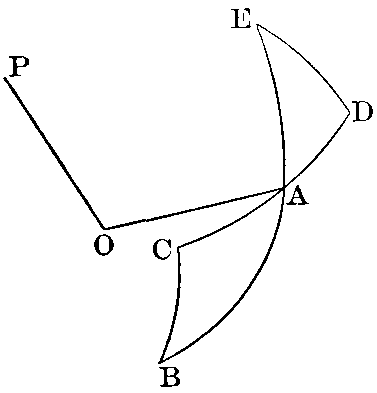
\includegraphics[width=40mm]{fig25.png}
\end{center}

To prove that $\beta^b \rho$ coincides with the axis of
$\beta^\frac{-b}{2} \rho^\frac{\pi}{2} \beta^\frac{b}{2}$. Take the
more general versor $\rho^\theta$. Let $OP$ represent the axis
$\beta$, $AB$ the versor $\beta^\frac{-b}{2}$, $BC$ the versor
$\rho^\theta$. Then $(AB)(BC) = AC = DA$, therefore $(AB)(BC)(AE) =
(DA)(AE) = DE$. Now $DE$ has the same angle as $BC$, but its axis
has been rotated round $P$ by the angle $b$. Hence if $\theta =
\frac{\pi}{2}$, the axis of $\beta^\frac{-b}{2}
\rho^\frac{\pi}{2}\beta^\frac{b}{2}$ will coincide with
$\beta^b\rho$.\footnote{This theorem was discovered by
Cayley.\index{Cayley} It indicates that quaternion multiplication in
the most general sense has its physical meaning in the composition
of rotations.}

The exponential expression for $\beta^\frac{-b}{2}
\rho^\frac{\pi}{2} \beta^\frac{b}{2}$ is
$e^{-\frac{1}{2}b\beta^\frac{\pi}{2} +
\frac{1}{2}\pi\rho^\frac{\pi}{2} + \frac{1}{2}b\beta^\frac{\pi}{2}}$
which may be expanded according to the exponential theorem, the
successive powers of the trinomial being formed according to the
multinomial theorem, the order of the factors being preserved.

\medskip Composition of Finite Rotations round Axes which
Intersect.---Let $\beta$ and $\gamma$ denote the two axes in space
round which the successive rotations take place, and let $\beta^b$
denote the first and $\gamma^c$ the second. Let $\beta^b \times
\gamma^c$ denote the single rotation which is equivalent to the two
given rotations applied in succession; the sign $\times$ is
introduced to distinguish from the product of versors. It has been
shown in the preceding paragraph that
\begin{gather*}
\beta^b\rho = \beta^\frac{-b}{2}\rho^\frac{\pi}{2}\beta^\frac{b}{2}; \\
\intertext{and as the result is a line, the same principle applies
to the subsequent rotation. Hence}
\begin{split}
\gamma^c(\beta^b\rho) &=
  \gamma^\frac{-c}{2}(\beta^\frac{-b}{2}\rho^\frac{\pi}{2}
     \beta^\frac{\pi}{2})\gamma^\frac{c}{2} \\
&= (\gamma^\frac{-c}{2}\beta^\frac{-b}{2})
     \rho^\frac{\pi}{2} (\beta^\frac{b}{2}\gamma^\frac{c}{2}),
\end{split} \\
\intertext{because the factors in a product of versors can be
associated in any manner. Hence, reasoning backwards,}
\beta^b \times \gamma^c = (\beta^\frac{b}{2}\gamma^\frac{c}{2})^2. \\
\intertext{Let $m$ denote the cosine of
$\beta^\frac{b}{2}\gamma^\frac{c}{2}$, namely,}
\cos\frac{b}{2}\,\cos\frac{c}{2}-\sin\frac{b}{2}\,\sin\frac{c}{2}, \\
\intertext{ and $n \cdot \nu$ their directed sine, namely,}
\cos \frac{b}{2}\, \sin \frac{c}{2} \cdot \gamma + \cos\frac{c}{2}\,
\sin \frac{b}{2} \cdot \beta - \sin \frac{b}{2}\,
  \sin \frac{c}{2}\, \sin \beta\gamma \cdot \overline{\beta\gamma}; \\
\intertext{then}
\beta^b \times \gamma^c = m^2 - n^2 + 2mn \cdot \nu.
\end{gather*}

\newpage
\begin{center}
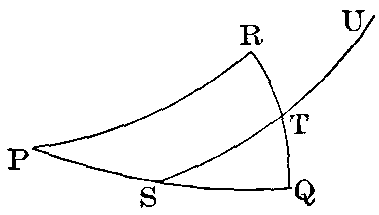
\includegraphics[width=40mm]{fig26.png}
\end{center}

\smallskip Observation.---The expression
$(\beta^\frac{b}{2}\gamma^\frac{c}{2})^2$ is not, as might be
supposed, identical with $\beta^b\gamma^c$. The former reduces to
the latter only when $\beta$ and $\gamma$ are the same or opposite.
In the figure $\beta^b$ is represented by $PQ$, $\gamma^c$ by $QR$,
$\beta^b\gamma^c$ by $PR$, $\beta^\frac{b}{2}\gamma^\frac{c}{2}$ by
$ST$, and $(\beta^\frac{b}{2}\gamma^\frac{c}{2})^2$ by $SU$, which
is twice $ST$. The cosine of $SU$ differs from the cosine of $PR$ by
the term $-(\sin \frac{b}{2}\, \sin \frac{c}{2}\, \sin
\beta\gamma)^2$ It is evident from the figure that their axes are
also different.

\medskip Corollary.---When $b$ and $c$ are infinitesimals,
$\cos\beta^b \times \gamma^c = 1$, and $\Sin \beta^b \times \gamma^c
= b \cdot \beta + c \cdot \gamma$, which is the parallelogram rule
for the composition of infinitesimal rotations.

\small \begin{enumerate}

\item[Prob.~54.] Let $\beta = \overline{30^\circ/}\!
\underline{/45^\circ}$, $\theta = \frac{\pi}{3}$, and $R = 2i - 3j +
4k$; calculate $\beta^\theta R$.

\item[Prob.~55.] Let $\beta = \overline{90^\circ/}\!
\underline{/90^\circ}$, $\theta = \frac{\pi}{4}$, $R = -i + 2j -
3k$; calculate $\beta^\theta R$.

\item[Prob.~56.] Prove by multiplying out that $\beta^\frac{-b}{2}
\rho^\frac{\pi}{2} \beta^\frac{b}{2} =
\{\beta^b\rho\}^\frac{\pi}{2}$.

\item[Prob.~57.] Prove by means of the exponential theorem that
$\gamma^{-c}\beta^b\gamma^c$ has an angle $b$, and that its axis is
$\gamma^{2c}\beta$.

\item[Prob.~58.] Prove that the cosine of
$(\beta^\frac{b}{2}\gamma^\frac{c}{2})^2$
differs from the cosine of $\beta^b\gamma^c$ by \\
$-(\sin\frac{b}{2} \sin\frac{c}{2} \sin\beta \gamma)^2$.

\item[Prob.~59.] Compare the axes of
$(\beta^\frac{b}{2}\gamma^\frac{c}{2})^2$ and $\beta^b\gamma^c$.

\item[Prob.~60.] Find the value of $\beta^b\times\gamma^c$ when
$\beta = \overline{0^\circ/}\!\underline{/90^\circ}$ and
$\gamma=\overline{90^\circ/}\!\underline{/90^\circ}$.

\item[Prob.~61.] Find the single rotation equivalent to
$i^\frac{\pi}{2} \times j^\frac{\pi}{2} \times k^\frac{\pi}{2}$.

\item[Prob.~62.] Prove that successive rotations about radii to two
corners of a spherical triangle and through angles double of those
of the triangle are equivalent to a single rotation about the radius
to the third corner, and through an angle double of the external
angle of the triangle.
\end{enumerate} \normalsize

\addcontentsline{toc}{chapter}{Index}
\printindex

\markright{ADVERTISEMENT}
\begin{center}
\textbf{
\Large SHORT-TITLE CATALOGUE \\
\small OF THE           \\
\Large PUBLICATIONS          \\
\small OF               \\
\Large JOHN WILEY \& SONS, \textsc{Inc.} \\
\normalsize NEW YORK  \\
London: CHAPMAN \& HALL, Limited \\
Montreal, Can.: RENOUF PUB. CO.} \\

\bigskip
\begin{center}
\rule{25mm}{.2pt}
\end{center}
\medskip
\normalsize \textbf{ARRANGED UNDER SUBJECTS} \\
\footnotesize Descriptive circulars sent on application. Books
marked with an asterisk (*) are sold at \emph{net} prices only. All
books are bound in cloth unless otherwise stated.

\medskip
\begin{center}
\rule{25mm}{.2pt}
\end{center}
\bigskip

\normalsize
\textbf{AGRICULTURE---HORTICULTURE---FORESTRY.}
\bigskip

{\footnotesize
\begin{tabular}{lr}
\textsc{Armsby}---Principles of Animal Nutrition \dotfill 8vo,
                                                          & \$4 00 \\
\textsc{Bowman}---Forest Physiography \dotfill 8vo, & *5 00 \\
\textsc{Bryant}---Hand Book of Logging\dotfill  (Ready, Fall 1913)
                                                                 & \\
\textsc{Budd} and \textsc{Hansen}---American Horticultural Manual:
                                                        \dotfill & \\
\quad Part I. Propagation, Culture, and Improvement\dotfill 12mo,
                                                            & 1 50 \\
\quad Part II. Systematic Pomology \dotfill 12mo, & 1 50 \\
\textsc{Elliott}---Engineering for Land Drainage \dotfill 12mo,
                                                            & 2 00 \\
\quad  Practical Farm Drainage.  (Second Edition, Rewritten)
                                             \dotfill 12mo, & 1 50 \\
\textsc{Fuller}---Domestic Water Supplies for the Farm \dotfill 8vo,
                                                           & *1 50 \\
\textsc{Graham}---Text-book on Poultry \dotfill
                                        (\emph{In Preparation.}) & \\
\quad  Manual on Poultry (Loose Leaf Lab. Manual)
  \dotfill (\emph{In Preparation.}) & \\
\textsc{Graves}---Forest Mensuration \dotfill 8vo, & 4 00 \\
\quad  Principles of Handling Woodlands \dotfill Small 8vo,
                                                           & *1 50 \\
\textsc{Green}---Principles of American Forestry \dotfill 12mo,
                                                            & 1 50 \\
\textsc{Grotenfelt}---Principles of Modern Dairy Practice.
(\textsc{Woll}.) \dotfill 12mo, & 2 00 \\
\textsc{Hawley} and \textsc{Hawes}---Forestry in New England
\dotfill  8vo, & *3 50 \\
\textsc{Herrick}---Denatured or Industrial Alcohol \dotfill 8vo,
                                                           & *4 00 \\
\textsc{Howe}---Agricultural Drafting \dotfill oblong quarto,
                                                           & *1 25 \\
\quad Reference and Problem Sheets to accompany
                      Agricultural Drafting, \dotfill each & *0 20 \\
\textsc{Keitt}---Agricultural Chemistry Text-book
   \dotfill (\emph{In Preparation.}) & \\
\quad Laboratory and Field Exercises in Agricultural Chemistry
  \dotfill (\emph{In Preparation.}) & \\
\textsc{Kemp} and \textsc{Waugh}---Landscape Gardening. (New
Edition, Rewritten)
  \dotfill  12mo, & *1 50 \\
\textsc{Larsen}---Exercises in Dairying (Loose Leaf Field Manual)
  \dotfill 4to, paper, & *1 00 \\
\quad  Single Exercises each \dotfill &  *0 02 \\
\quad  and \textsc{White}---Dairy Technology \dotfill Small 8vo,
                                                           & *1 50 \\
\textsc{Levison}---Studies of Trees, Loose Leaf Field Manual, 4to,
  pamphlet form,  & \\
\quad  Price from 5--10 cents net, each, according to number
                                                       of pages. & \\
\textsc{McCall}---Crops and Soils (Loose Leaf Field Manual)
  \dotfill (\emph{In Preparation.}) & \\
\quad  Soils (Text-book) \dotfill (\emph{In Preparation.}) & \\
\textsc{McKay} and \textsc{Larsen}---Principles and Practice of
                               Butter-making \dotfill 8vo, & *1 50 \\
\textsc{Maynard}---Landscape Gardening as Applied to Home Decoration
  \dotfill 12mo, & 1 50 \\
\textsc{Moon} and \textsc{Brown}---Elements of Forestry
  \dotfill (\emph{In Preparation.}) & \\
\textsc{Record}---Identification of the Economic Woods of the United
States \dotfill 8vo, & *1 25 \\
\textsc{Recknagel}---Theory and Practice of Working Plans (Forest
  Organization) \dotfill 8vo, & *2 00
\end{tabular}
} % \end{\footnotesize}
\end{center}
\newpage
\chapter{PROJECT GUTENBERG ``SMALL PRINT''}
\small \pagenumbering{gobble}
\begin{verbatim}

End of the Project Gutenberg EBook of Vector Analysis and Quaternions, 
by Alexander Macfarlane

*** END OF THIS PROJECT GUTENBERG EBOOK VECTOR ANALYSIS AND QUATERNIONS ***

***** This file should be named 13609-t.tex or 13609-t.zip *****
This and all associated files of various formats will be found in:
        http://www.gutenberg.net/1/3/6/0/13609/

Produced by David Starner, Joshua Hutchinson, John Hagerson, and the 
Project Gutenberg On-line Distributed Proofreaders.



Updated editions will replace the previous one--the old editions
will be renamed.

Creating the works from public domain print editions means that no
one owns a United States copyright in these works, so the Foundation
(and you!) can copy and distribute it in the United States without
permission and without paying copyright royalties.  Special rules,
set forth in the General Terms of Use part of this license, apply to
copying and distributing Project Gutenberg-tm electronic works to
protect the PROJECT GUTENBERG-tm concept and trademark.  Project
Gutenberg is a registered trademark, and may not be used if you
charge for the eBooks, unless you receive specific permission.  If
you do not charge anything for copies of this eBook, complying with
the rules is very easy.  You may use this eBook for nearly any
purpose such as creation of derivative works, reports, performances
and research.  They may be modified and printed and given away--you
may do practically ANYTHING with public domain eBooks.
Redistribution is subject to the trademark license, especially
commercial redistribution.



*** START: FULL LICENSE ***

THE FULL PROJECT GUTENBERG LICENSE PLEASE READ THIS BEFORE YOU
DISTRIBUTE OR USE THIS WORK

To protect the Project Gutenberg-tm mission of promoting the free
distribution of electronic works, by using or distributing this work
(or any other work associated in any way with the phrase "Project
Gutenberg"), you agree to comply with all the terms of the Full
Project Gutenberg-tm License (available with this file or online at
http://gutenberg.net/license).


Section 1.  General Terms of Use and Redistributing Project
Gutenberg-tm electronic works

1.A.  By reading or using any part of this Project Gutenberg-tm
electronic work, you indicate that you have read, understand, agree
to and accept all the terms of this license and intellectual
property (trademark/copyright) agreement.  If you do not agree to
abide by all the terms of this agreement, you must cease using and
return or destroy all copies of Project Gutenberg-tm electronic
works in your possession. If you paid a fee for obtaining a copy of
or access to a Project Gutenberg-tm electronic work and you do not
agree to be bound by the terms of this agreement, you may obtain a
refund from the person or entity to whom you paid the fee as set
forth in paragraph 1.E.8.

1.B.  "Project Gutenberg" is a registered trademark.  It may only be
used on or associated in any way with an electronic work by people
who agree to be bound by the terms of this agreement.  There are a
few things that you can do with most Project Gutenberg-tm electronic
works even without complying with the full terms of this agreement.
See paragraph 1.C below.  There are a lot of things you can do with
Project Gutenberg-tm electronic works if you follow the terms of
this agreement and help preserve free future access to Project
Gutenberg-tm electronic works.  See paragraph 1.E below.

1.C.  The Project Gutenberg Literary Archive Foundation ("the
Foundation" or PGLAF), owns a compilation copyright in the
collection of Project Gutenberg-tm electronic works.  Nearly all the
individual works in the collection are in the public domain in the
United States.  If an individual work is in the public domain in the
United States and you are located in the United States, we do not
claim a right to prevent you from copying, distributing, performing,
displaying or creating derivative works based on the work as long as
all references to Project Gutenberg are removed.  Of course, we hope
that you will support the Project Gutenberg-tm mission of promoting
free access to electronic works by freely sharing Project
Gutenberg-tm works in compliance with the terms of this agreement
for keeping the Project Gutenberg-tm name associated with the work.
You can easily comply with the terms of this agreement by keeping
this work in the same format with its attached full Project
Gutenberg-tm License when you share it without charge with others.

1.D.  The copyright laws of the place where you are located also
govern what you can do with this work.  Copyright laws in most
countries are in a constant state of change.  If you are outside the
United States, check the laws of your country in addition to the
terms of this agreement before downloading, copying, displaying,
performing, distributing or creating derivative works based on this
work or any other Project Gutenberg-tm work.  The Foundation makes
no representations concerning the copyright status of any work in
any country outside the United States.

1.E.  Unless you have removed all references to Project Gutenberg:

1.E.1.  The following sentence, with active links to, or other
immediate access to, the full Project Gutenberg-tm License must
appear prominently whenever any copy of a Project Gutenberg-tm work
(any work on which the phrase "Project Gutenberg" appears, or with
which the phrase "Project Gutenberg" is associated) is accessed,
displayed, performed, viewed, copied or distributed:

This eBook is for the use of anyone anywhere at no cost and with
almost no restrictions whatsoever.  You may copy it, give it away or
re-use it under the terms of the Project Gutenberg License included
with this eBook or online at www.gutenberg.net

1.E.2.  If an individual Project Gutenberg-tm electronic work is
derived from the public domain (does not contain a notice indicating
that it is posted with permission of the copyright holder), the work
can be copied and distributed to anyone in the United States without
paying any fees or charges.  If you are redistributing or providing
access to a work with the phrase "Project Gutenberg" associated with
or appearing on the work, you must comply either with the
requirements of paragraphs 1.E.1 through 1.E.7 or obtain permission
for the use of the work and the Project Gutenberg-tm trademark as
set forth in paragraphs 1.E.8 or 1.E.9.

1.E.3.  If an individual Project Gutenberg-tm electronic work is
posted with the permission of the copyright holder, your use and
distribution must comply with both paragraphs 1.E.1 through 1.E.7
and any additional terms imposed by the copyright holder.
Additional terms will be linked to the Project Gutenberg-tm License
for all works posted with the permission of the copyright holder
found at the beginning of this work.

1.E.4.  Do not unlink or detach or remove the full Project
Gutenberg-tm License terms from this work, or any files containing a
part of this work or any other work associated with Project
Gutenberg-tm.

1.E.5.  Do not copy, display, perform, distribute or redistribute
this electronic work, or any part of this electronic work, without
prominently displaying the sentence set forth in paragraph 1.E.1
with active links or immediate access to the full terms of the
Project Gutenberg-tm License.

1.E.6.  You may convert to and distribute this work in any binary,
compressed, marked up, nonproprietary or proprietary form, including
any word processing or hypertext form.  However, if you provide
access to or distribute copies of a Project Gutenberg-tm work in a
format other than "Plain Vanilla ASCII" or other format used in the
official version posted on the official Project Gutenberg-tm web
site (www.gutenberg.net), you must, at no additional cost, fee or
expense to the user, provide a copy, a means of exporting a copy, or
a means of obtaining a copy upon request, of the work in its
original "Plain Vanilla ASCII" or other form.  Any alternate format
must include the full Project Gutenberg-tm License as specified in
paragraph 1.E.1.

1.E.7.  Do not charge a fee for access to, viewing, displaying,
performing, copying or distributing any Project Gutenberg-tm works
unless you comply with paragraph 1.E.8 or 1.E.9.

1.E.8.  You may charge a reasonable fee for copies of or providing
access to or distributing Project Gutenberg-tm electronic works
provided that

- You pay a royalty fee of 20% of the gross profits you derive from
     the use of Project Gutenberg-tm works calculated using the method
     you already use to calculate your applicable taxes.  The fee is
     owed to the owner of the Project Gutenberg-tm trademark, but he
     has agreed to donate royalties under this paragraph to the
     Project Gutenberg Literary Archive Foundation.  Royalty payments
     must be paid within 60 days following each date on which you
     prepare (or are legally required to prepare) your periodic tax
     returns.  Royalty payments should be clearly marked as such and
     sent to the Project Gutenberg Literary Archive Foundation at the
     address specified in Section 4, "Information about donations to
     the Project Gutenberg Literary Archive Foundation."

- You provide a full refund of any money paid by a user who notifies
     you in writing (or by e-mail) within 30 days of receipt that s/he
     does not agree to the terms of the full Project Gutenberg-tm
     License.  You must require such a user to return or
     destroy all copies of the works possessed in a physical medium
     and discontinue all use of and all access to other copies of
     Project Gutenberg-tm works.

- You provide, in accordance with paragraph 1.F.3, a full refund of
     any money paid for a work or a replacement copy, if a defect in
     the electronic work is discovered and reported to you within 90
     days of receipt of the work.

- You comply with all other terms of this agreement for free
     distribution of Project Gutenberg-tm works.

1.E.9.  If you wish to charge a fee or distribute a Project
Gutenberg-tm electronic work or group of works on different terms
than are set forth in this agreement, you must obtain permission in
writing from both the Project Gutenberg Literary Archive Foundation
and Michael Hart, the owner of the Project Gutenberg-tm trademark.
Contact the Foundation as set forth in Section 3 below.

1.F.

1.F.1.  Project Gutenberg volunteers and employees expend
considerable effort to identify, do copyright research on,
transcribe and proofread public domain works in creating the Project
Gutenberg-tm collection.  Despite these efforts, Project
Gutenberg-tm electronic works, and the medium on which they may be
stored, may contain "Defects," such as, but not limited to,
incomplete, inaccurate or corrupt data, transcription errors, a
copyright or other intellectual property infringement, a defective
or damaged disk or other medium, a computer virus, or computer codes
that damage or cannot be read by your equipment.

1.F.2.  LIMITED WARRANTY, DISCLAIMER OF DAMAGES - Except for the
"Right of Replacement or Refund" described in paragraph 1.F.3, the
Project Gutenberg Literary Archive Foundation, the owner of the
Project Gutenberg-tm trademark, and any other party distributing a
Project Gutenberg-tm electronic work under this agreement, disclaim
all liability to you for damages, costs and expenses, including
legal fees.  YOU AGREE THAT YOU HAVE NO REMEDIES FOR NEGLIGENCE,
STRICT LIABILITY, BREACH OF WARRANTY OR BREACH OF CONTRACT EXCEPT
THOSE PROVIDED IN PARAGRAPH F3.  YOU AGREE THAT THE FOUNDATION, THE
TRADEMARK OWNER, AND ANY DISTRIBUTOR UNDER THIS AGREEMENT WILL NOT
BE LIABLE TO YOU FOR ACTUAL, DIRECT, INDIRECT, CONSEQUENTIAL,
PUNITIVE OR INCIDENTAL DAMAGES EVEN IF YOU GIVE NOTICE OF THE
POSSIBILITY OF SUCH DAMAGE.

1.F.3.  LIMITED RIGHT OF REPLACEMENT OR REFUND - If you discover a
defect in this electronic work within 90 days of receiving it, you
can receive a refund of the money (if any) you paid for it by
sending a written explanation to the person you received the work
from.  If you received the work on a physical medium, you must
return the medium with your written explanation.  The person or
entity that provided you with the defective work may elect to
provide a replacement copy in lieu of a refund.  If you received the
work electronically, the person or entity providing it to you may
choose to give you a second opportunity to receive the work
electronically in lieu of a refund.  If the second copy is also
defective, you may demand a refund in writing without further
opportunities to fix the problem.

1.F.4.  Except for the limited right of replacement or refund set
forth in paragraph 1.F.3, this work is provided to you 'AS-IS', WITH
NO OTHER WARRANTIES OF ANY KIND, EXPRESS OR IMPLIED, INCLUDING BUT
NOT LIMITED TO WARRANTIES OF MERCHANTIBILITY OR FITNESS FOR ANY
PURPOSE.

1.F.5.  Some states do not allow disclaimers of certain implied
warranties or the exclusion or limitation of certain types of
damages. If any disclaimer or limitation set forth in this agreement
violates the law of the state applicable to this agreement, the
agreement shall be interpreted to make the maximum disclaimer or
limitation permitted by the applicable state law.  The invalidity or
unenforceability of any provision of this agreement shall not void
the remaining provisions.

1.F.6.  INDEMNITY - You agree to indemnify and hold the Foundation,
the trademark owner, any agent or employee of the Foundation, anyone
providing copies of Project Gutenberg-tm electronic works in
accordance with this agreement, and any volunteers associated with
the production, promotion and distribution of Project Gutenberg-tm
electronic works, harmless from all liability, costs and expenses,
including legal fees, that arise directly or indirectly from any of
the following which you do or cause to occur: (a) distribution of
this or any Project Gutenberg-tm work, (b) alteration, modification,
or additions or deletions to any Project Gutenberg-tm work, and (c)
any Defect you cause.


Section  2.  Information about the Mission of Project Gutenberg-tm

Project Gutenberg-tm is synonymous with the free distribution of
electronic works in formats readable by the widest variety of
computers including obsolete, old, middle-aged and new computers.
It exists because of the efforts of hundreds of volunteers and
donations from people in all walks of life.

Volunteers and financial support to provide volunteers with the
assistance they need, is critical to reaching Project Gutenberg-tm's
goals and ensuring that the Project Gutenberg-tm collection will
remain freely available for generations to come.  In 2001, the
Project Gutenberg Literary Archive Foundation was created to provide
a secure and permanent future for Project Gutenberg-tm and future
generations. To learn more about the Project Gutenberg Literary
Archive Foundation and how your efforts and donations can help, see
Sections 3 and 4 and the Foundation web page at
http://www.pglaf.org.


Section 3.  Information about the Project Gutenberg Literary Archive
Foundation

The Project Gutenberg Literary Archive Foundation is a non profit
501(c)(3) educational corporation organized under the laws of the
state of Mississippi and granted tax exempt status by the Internal
Revenue Service.  The Foundation's EIN or federal tax identification
number is 64-6221541.  Its 501(c)(3) letter is posted at
http://pglaf.org/fundraising.  Contributions to the Project
Gutenberg Literary Archive Foundation are tax deductible to the full
extent permitted by U.S. federal laws and your state's laws.

The Foundation's principal office is located at 4557 Melan Dr. S.
Fairbanks, AK, 99712., but its volunteers and employees are
scattered throughout numerous locations.  Its business office is
located at 809 North 1500 West, Salt Lake City, UT 84116, (801)
596-1887, email business@pglaf.org.  Email contact links and up to
date contact information can be found at the Foundation's web site
and official page at http://pglaf.org

For additional contact information:
     Dr. Gregory B. Newby
     Chief Executive and Director
     gbnewby@pglaf.org

Section 4.  Information about Donations to the Project Gutenberg
Literary Archive Foundation

Project Gutenberg-tm depends upon and cannot survive without wide
spread public support and donations to carry out its mission of
increasing the number of public domain and licensed works that can
be freely distributed in machine readable form accessible by the
widest array of equipment including outdated equipment.  Many small
donations ($1 to $5,000) are particularly important to maintaining
tax exempt status with the IRS.

The Foundation is committed to complying with the laws regulating
charities and charitable donations in all 50 states of the United
States.  Compliance requirements are not uniform and it takes a
considerable effort, much paperwork and many fees to meet and keep
up with these requirements.  We do not solicit donations in
locations where we have not received written confirmation of
compliance.  To SEND DONATIONS or determine the status of compliance
for any particular state visit http://pglaf.org

While we cannot and do not solicit contributions from states where
we have not met the solicitation requirements, we know of no
prohibition against accepting unsolicited donations from donors in
such states who approach us with offers to donate.

International donations are gratefully accepted, but we cannot make
any statements concerning tax treatment of donations received from
outside the United States.  U.S. laws alone swamp our small staff.

Please check the Project Gutenberg Web pages for current donation
methods and addresses.  Donations are accepted in a number of other
ways including including checks, online payments and credit card
donations.  To donate, please visit: http://pglaf.org/donate


Section 5.  General Information About Project Gutenberg-tm
electronic works.

Professor Michael S. Hart is the originator of the Project
Gutenberg-tm concept of a library of electronic works that could be
freely shared with anyone.  For thirty years, he produced and
distributed Project Gutenberg-tm eBooks with only a loose network of
volunteer support.

Project Gutenberg-tm eBooks are often created from several printed
editions, all of which are confirmed as Public Domain in the U.S.
unless a copyright notice is included.  Thus, we do not necessarily
keep eBooks in compliance with any particular paper edition.

Most people start at our Web site which has the main PG search
facility:

     http://www.gutenberg.net

This Web site includes information about Project Gutenberg-tm,
including how to make donations to the Project Gutenberg Literary
Archive Foundation, how to help produce our new eBooks, and how to
subscribe to our email newsletter to hear about new eBooks.
\end{verbatim}

\end{document}
